\documentclass{article}

\usepackage{fancyhdr}
\usepackage{extramarks}
\usepackage{amsmath}
\usepackage{amsthm}
\usepackage{amsfonts}
\usepackage{tikz}
\usepackage[plain]{algorithm}
\usepackage{algpseudocode}
\usepackage{enumerate}
\usepackage{tikz}
\usepackage{dsfont}

\usetikzlibrary{automata,positioning}

%
% Basic Document Settings
%

\topmargin=-0.45in
\evensidemargin=0in
\oddsidemargin=0in
\textwidth=6.5in
\textheight=9.0in
\headsep=0.25in

\linespread{1.1}

\pagestyle{fancy}
\lhead{\hmwkAuthorName}
\chead{\hmwkClass : \hmwkTitle}
\rhead{\firstxmark}
\lfoot{\lastxmark}
\cfoot{\thepage}

\renewcommand\headrulewidth{0.4pt}
\renewcommand\footrulewidth{0.4pt}

\setlength\parindent{0pt}

%
% Create Problem Sections
%

\newcommand{\enterProblemHeader}[1]{
    \nobreak\extramarks{}{Problem \arabic{#1} continued on next page\ldots}\nobreak{}
    \nobreak\extramarks{Problem \arabic{#1} (continued)}{Problem \arabic{#1} continued on next page\ldots}\nobreak{}
}

\newcommand{\exitProblemHeader}[1]{
    \nobreak\extramarks{Problem \arabic{#1} (continued)}{Problem \arabic{#1} continued on next page\ldots}\nobreak{}
    \stepcounter{#1}
    \nobreak\extramarks{Problem \arabic{#1}}{}\nobreak{}
}

\newcommand*\circled[1]{\tikz[baseline=(char.base)]{
		\node[shape=circle,draw,inner sep=2pt] (char) {#1};}}


\setcounter{secnumdepth}{0}
\newcounter{partCounter}
\newcounter{homeworkProblemCounter}
\setcounter{homeworkProblemCounter}{1}
\nobreak\extramarks{Problem \arabic{homeworkProblemCounter}}{}\nobreak{}

%
% Homework Problem Environment
%
% This environment takes an optional argument. When given, it will adjust the
% problem counter. This is useful for when the problems given for your
% assignment aren't sequential. See the last 3 problems of this template for an
% example.
%

\newenvironment{homeworkProblem}[1][-1]{
    \ifnum#1>0
        \setcounter{homeworkProblemCounter}{#1}
    \fi
    \section{Problem \arabic{homeworkProblemCounter}}
    \setcounter{partCounter}{1}
    \enterProblemHeader{homeworkProblemCounter}
}{
    \exitProblemHeader{homeworkProblemCounter}
}

%
% Homework Details
%   - Title
%   - Class
%   - Due date
%   - Name
%   - Student ID

\newcommand{\hmwkTitle}{Homework\ \#01}
% \newcommand{\hmwkTitle}{Homework\\ \circled{1}}
\newcommand{\hmwkClass}{SI252 Reinforcement Learning}
\newcommand{\hmwkDueDate}{March 9, 2025}
\newcommand{\hmwkAuthorName}{Zhou Shouchen}
\newcommand{\hmwkAuthorID}{2021533042}


%
% Title Page
%

\title{
    \vspace{2in}
    \textmd{\textbf{\hmwkClass:\\  \hmwkTitle}} \\
    \normalsize\vspace{0.1in}\small{Due\ on\ \hmwkDueDate\ at 11:59 a.m.(CST)} \\
	\vspace{4in}
}

\author{
	Name: \textbf{\hmwkAuthorName} \\
	Student ID: \hmwkAuthorID}
\date{}

\renewcommand{\part}[1]{\textbf{\large Part \Alph{partCounter}}\stepcounter{partCounter}\\}

%
% Various Helper Commands
%

% Useful for algorithms
\newcommand{\alg}[1]{\textsc{\bfseries \footnotesize #1}}
% For derivatives
\newcommand{\deriv}[1]{\dfrac{\mathrm{d}}{\mathrm{d}x} (#1)}
% For partial derivatives
\newcommand{\pderiv}[2]{\dfrac{\partial}{\partial #1} (#2)}
% Integral dx
\newcommand{\dx}{\mathrm{d}x}
\newcommand{\du}{\mathrm{d}u}
\newcommand{\dr}{\mathrm{d}r}
\newcommand{\dS}{\mathrm{d}S}
\newcommand{\dtheta}{\mathrm{d}\theta}
\newcommand{\dphi}{\mathrm{d}\phi}

% Alias for the Solution section header
\newcommand{\solution}{\textcolor{blue}{\textbf{\large Solution}} \\}
% Probability commands: Expectation, Variance, Covariance, Bias
\newcommand{\E}{\mathbb{E}}
\newcommand{\Var}{\mathrm{Var}}
\newcommand{\Cov}{\mathrm{Cov}}
\newcommand{\Bias}{\mathrm{Bias}}
\newcommand{\Unif}{\operatorname{Unif}}
\newcommand{\Beta}{\operatorname{Beta}}
\newcommand{\Bin}{\operatorname{Bin}}
\newcommand{\N}{\mathcal{N}}
\newcommand{\I}{\mathds{1}}


\begin{document}

\maketitle
\pagebreak

\begin{homeworkProblem}

\textbf{Required: OpenAI Spinning Up in Deep RL}. Welcome to \href{https://spinningup.openai.com/en/latest/user/introduction.html}{Spinning Up in Deep RL}! This is an educational resource produced by OpenAI that makes it easier to learn about deep reinforcement learning (deep RL). Please study the documents and install the environment with PyTorch version.

(a) Finish the problem set 1: ``\href{https://spinningup.openai.com/en/latest/spinningup/exercises.html#problem-set-1-basics-of-implementation}{Basics of Implementation}". It includes three exercises: Gaussian Log-Likelihood, Policy for PPO, and Computation Graph for TD3.

(b) Finish the problem set 2: ``\href{https://spinningup.openai.com/en/latest/spinningup/exercises.html#problem-set-2-algorithm-failure-modes}{Algorithm Failure Modes}". It includes two exercises: Value Function Fitting in TRPO, and Silent Bug in DDPG.

\solution

(a) After setting up the environment in the methods in `README.md', we can successfully run the codes. The codes cuold be check in `code/spinningup/spinup/exercises/pytorch/problem\_set\_1'.

\begin{itemize}
    \item exercise 1\_1: For a $k$ dimension diagnoal Gaussian distribtion $\mathbf{x}\sim\N(\bmu,\bSigma)$, where $\bSigma=\diag(\sigma_1^2,\dots,\sigma_k^2)$, thus its PDF is
    $$p(\mathbf{x};\bmu,\bSigma)=\dfrac{1}{(2\pi)^{\frac{k}{2}}\,|\bSigma|^{\frac{1}{2}}}\exp\left[-\frac{1}{2}(\mathbf{x}-\bmu)^{\top}\bSigma^{-1}(\mathbf{x}\bmu)\right]$$
    Where
    $$|\bSigma|=\prod_{i=1}^{k}\sigma_i^{2}, \qquad \bSigma^{-1}=\diag\left(\sigma_1^{-2},\dots,\sigma_k^{-2}\right), \qquad (\mathbf{x}-\bmu)^{\top}\bSigma^{-1}(\mathbf{x}-\bmu)=\sum_{i=1}^{k}\frac{(x_i-\mu_i)^2}{\sigma_i^{2}}$$
    So above all, the log-likelihood is
    \begin{align*}
    \log p(\mathbf{x};\bmu,\bSigma) &= -\frac{k}{2}\log(2\pi)-\sum_{i=1}^{k}\log\sigma_i-\frac{1}{2}\sum_{i=1}^{k}\frac{(x_i-\mu_i)^2}{\sigma_i^{2}} \\
    &= -\dfrac{1}{2}\sum_{i=1}^k\left(\log(2\pi)+2\log\sigma_i+\left(\dfrac{x_i-\mu_i}{\sigma_i}\right)^2\right)
    \end{align*}

    The implementation are check results are as follows:
    \begin{figure}[h]
        \centering
        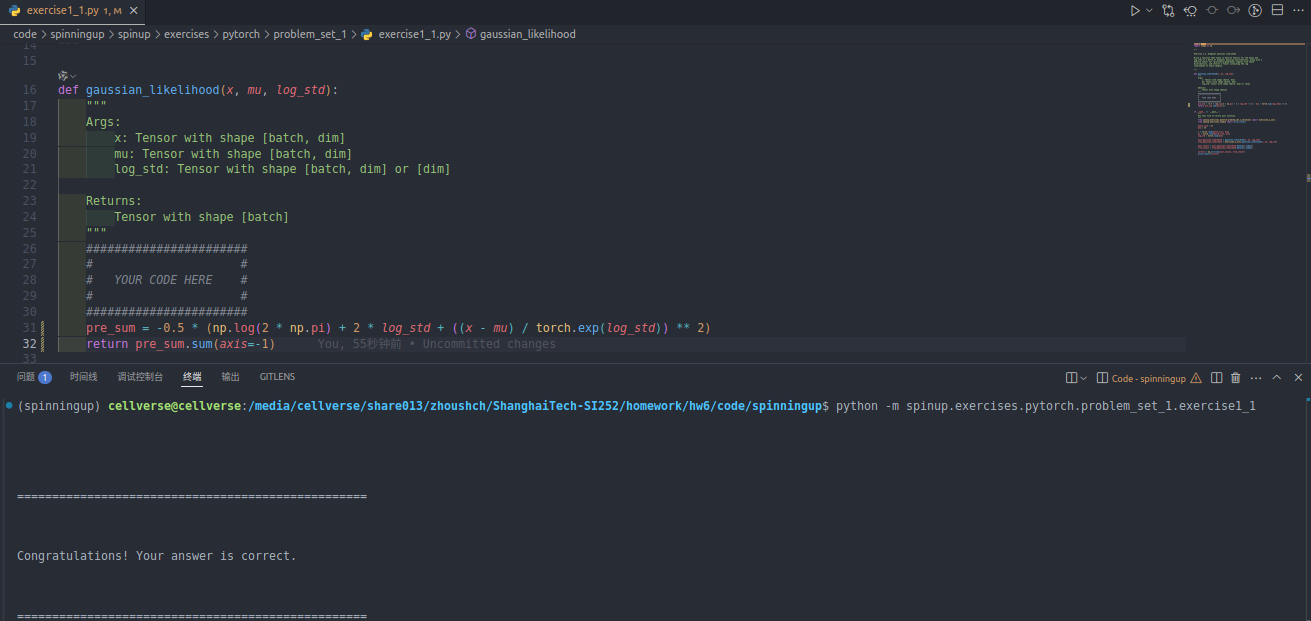
\includegraphics[width=\textwidth]{../Img/spinningup_exercises/1_1.png}
    \end{figure}

    \item exercise 1\_2: The implementation are check results are as follows:
    \begin{figure}[h]
        \centering
        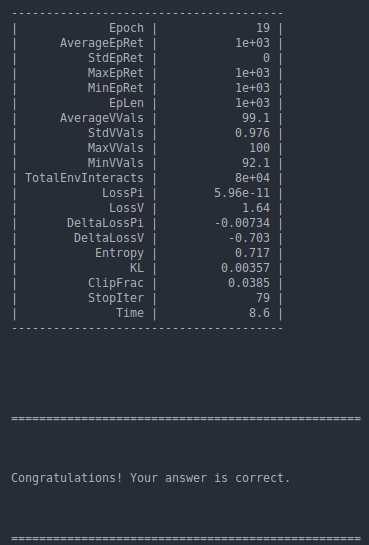
\includegraphics[width=0.5\textwidth]{../Img/spinningup_exercises/1_2.png}
    \end{figure}

    \item exercise 1\_3:
    According to the discription, within 10 rounds, the score in HalfSheetah should exceed 300, while the score in InvertedPendulum should reach 150.

    And the following curves show that the performance achieved the expected results:
    \begin{figure}[H]
        \centering
        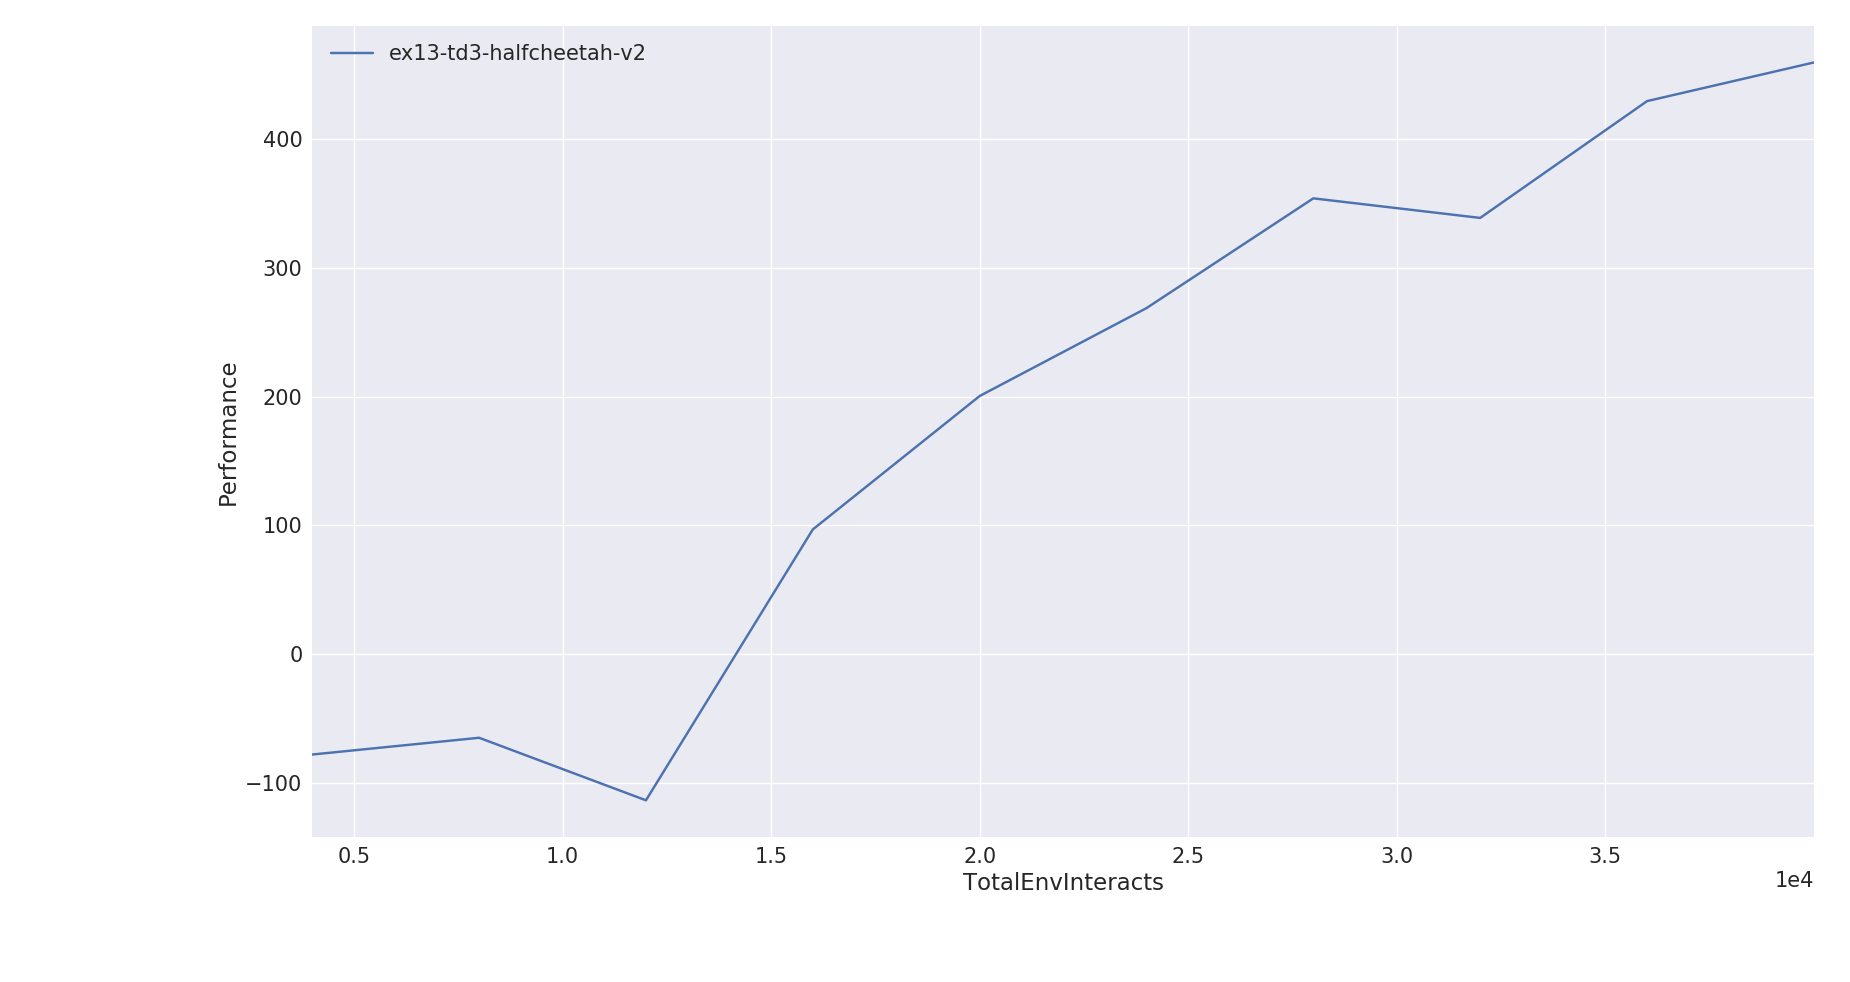
\includegraphics[width=\textwidth]{../Img/spinningup_exercises/1_3_healthcare.png}
        \vspace{-2cm}
    \end{figure}
    \begin{figure}[H]
        \centering
        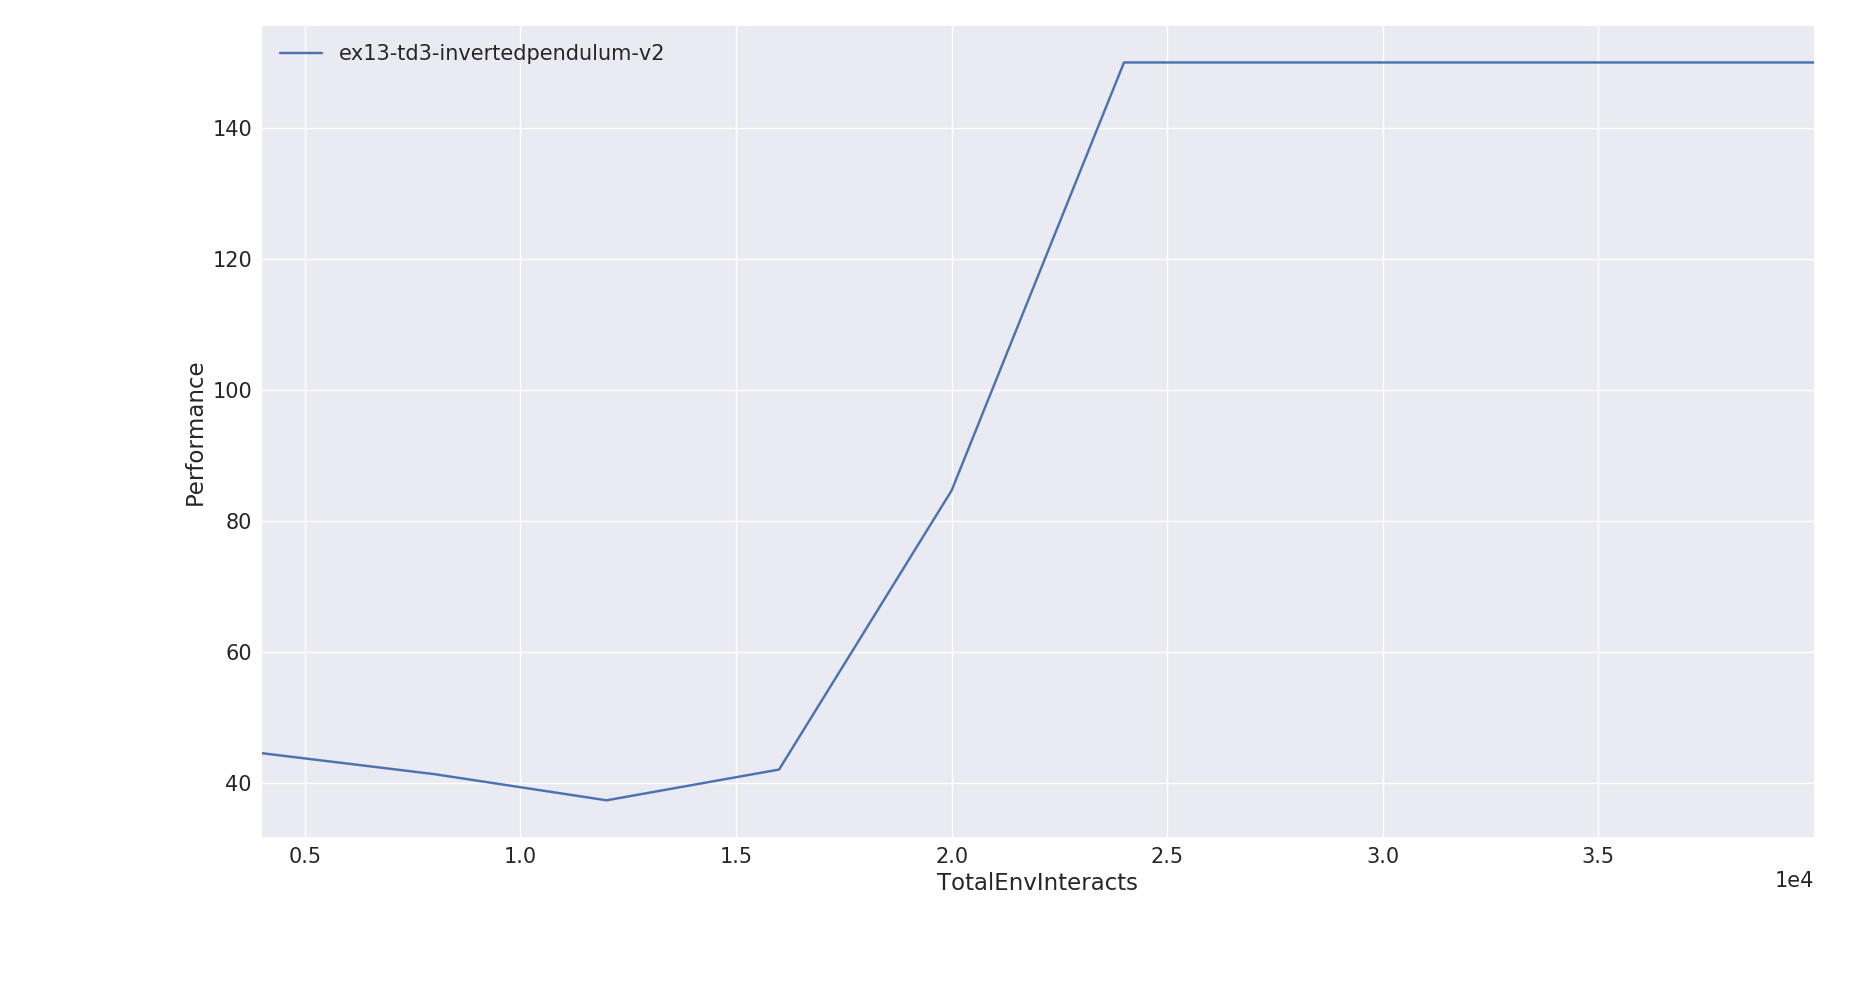
\includegraphics[width=\textwidth]{../Img/spinningup_exercises/1_3_invertedpendulum.png}
    \end{figure}

\end{itemize}


(b) Run the commands in the `README.md', we can get the following reults. The codes cuold be check in `code/spinningup/spinup/exercises/pytorch/problem\_set\_2'.

\begin{itemize}
    \item exercise 2\_1:

    The difference is quite substantial: with a trained value function, the agent is able to quickly make progress. With an untrained value function, the agent gets stuck early on.

    The curve of v0 with different seeds are as follows:
    \begin{figure}[H]
        \centering
        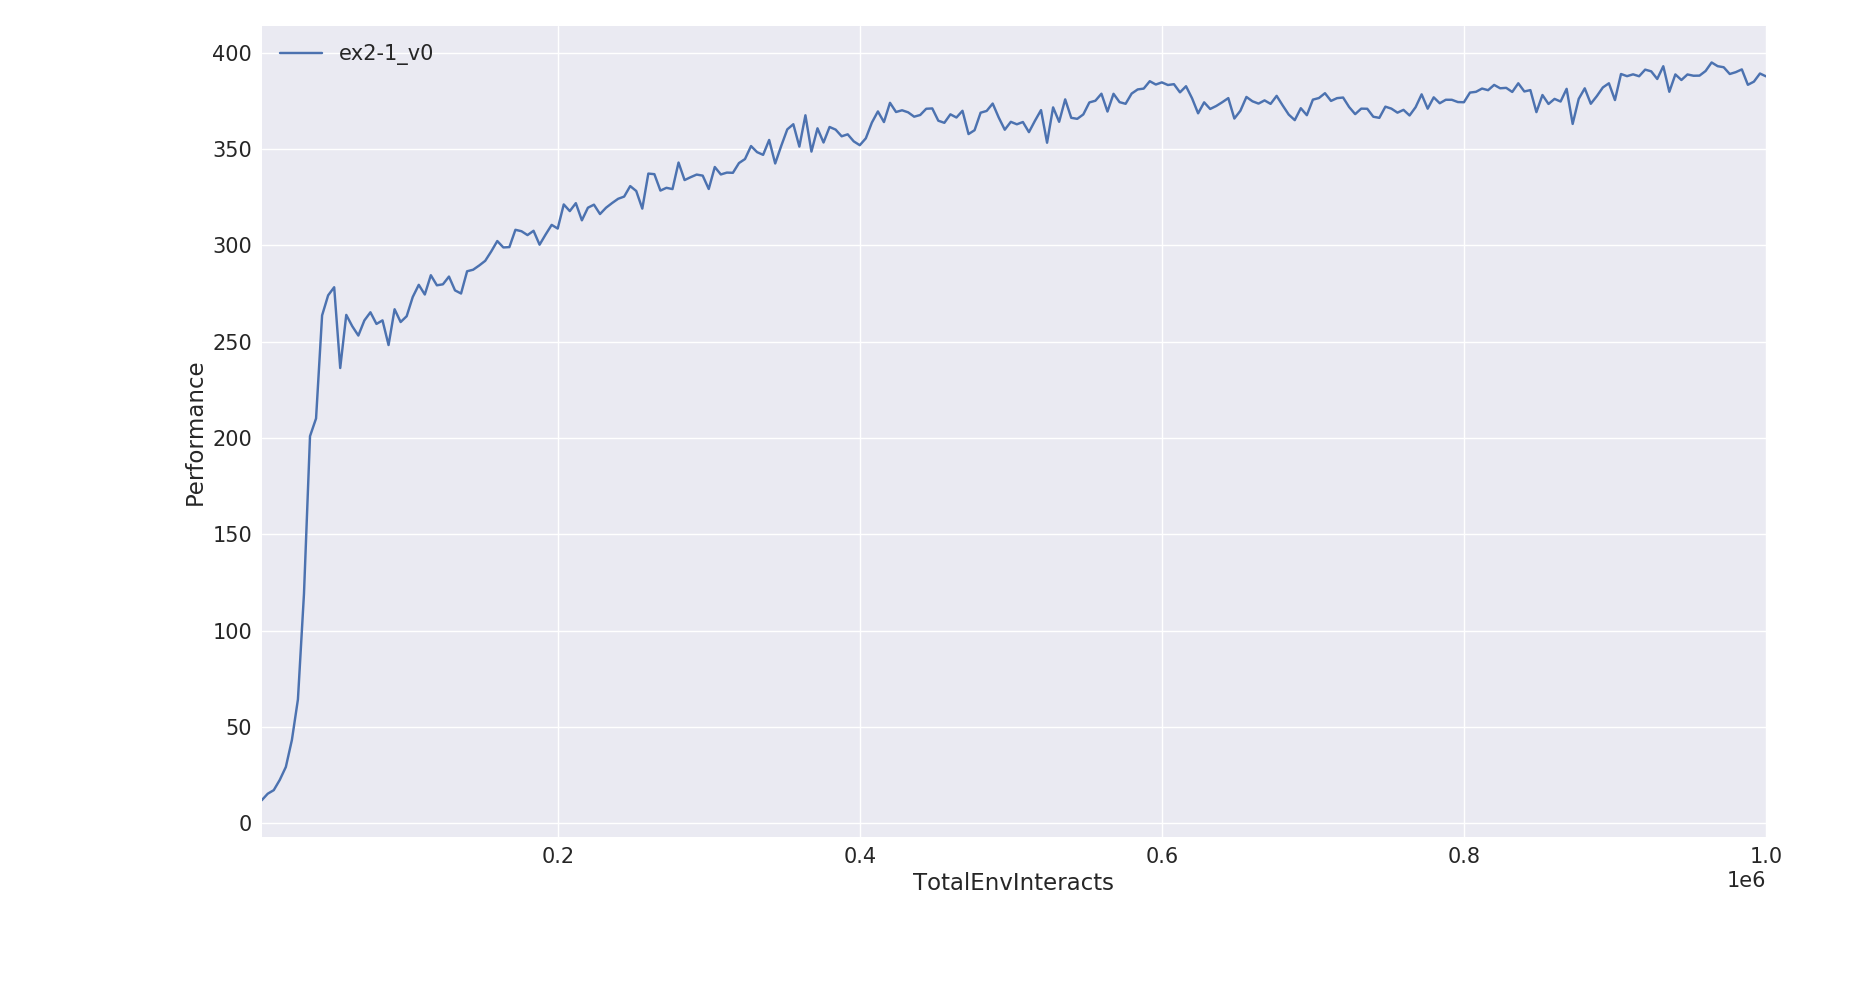
\includegraphics[width=0.32\textwidth]{../Img/spinningup_exercises/2_1/2_1_curve_v0_s0.png}
        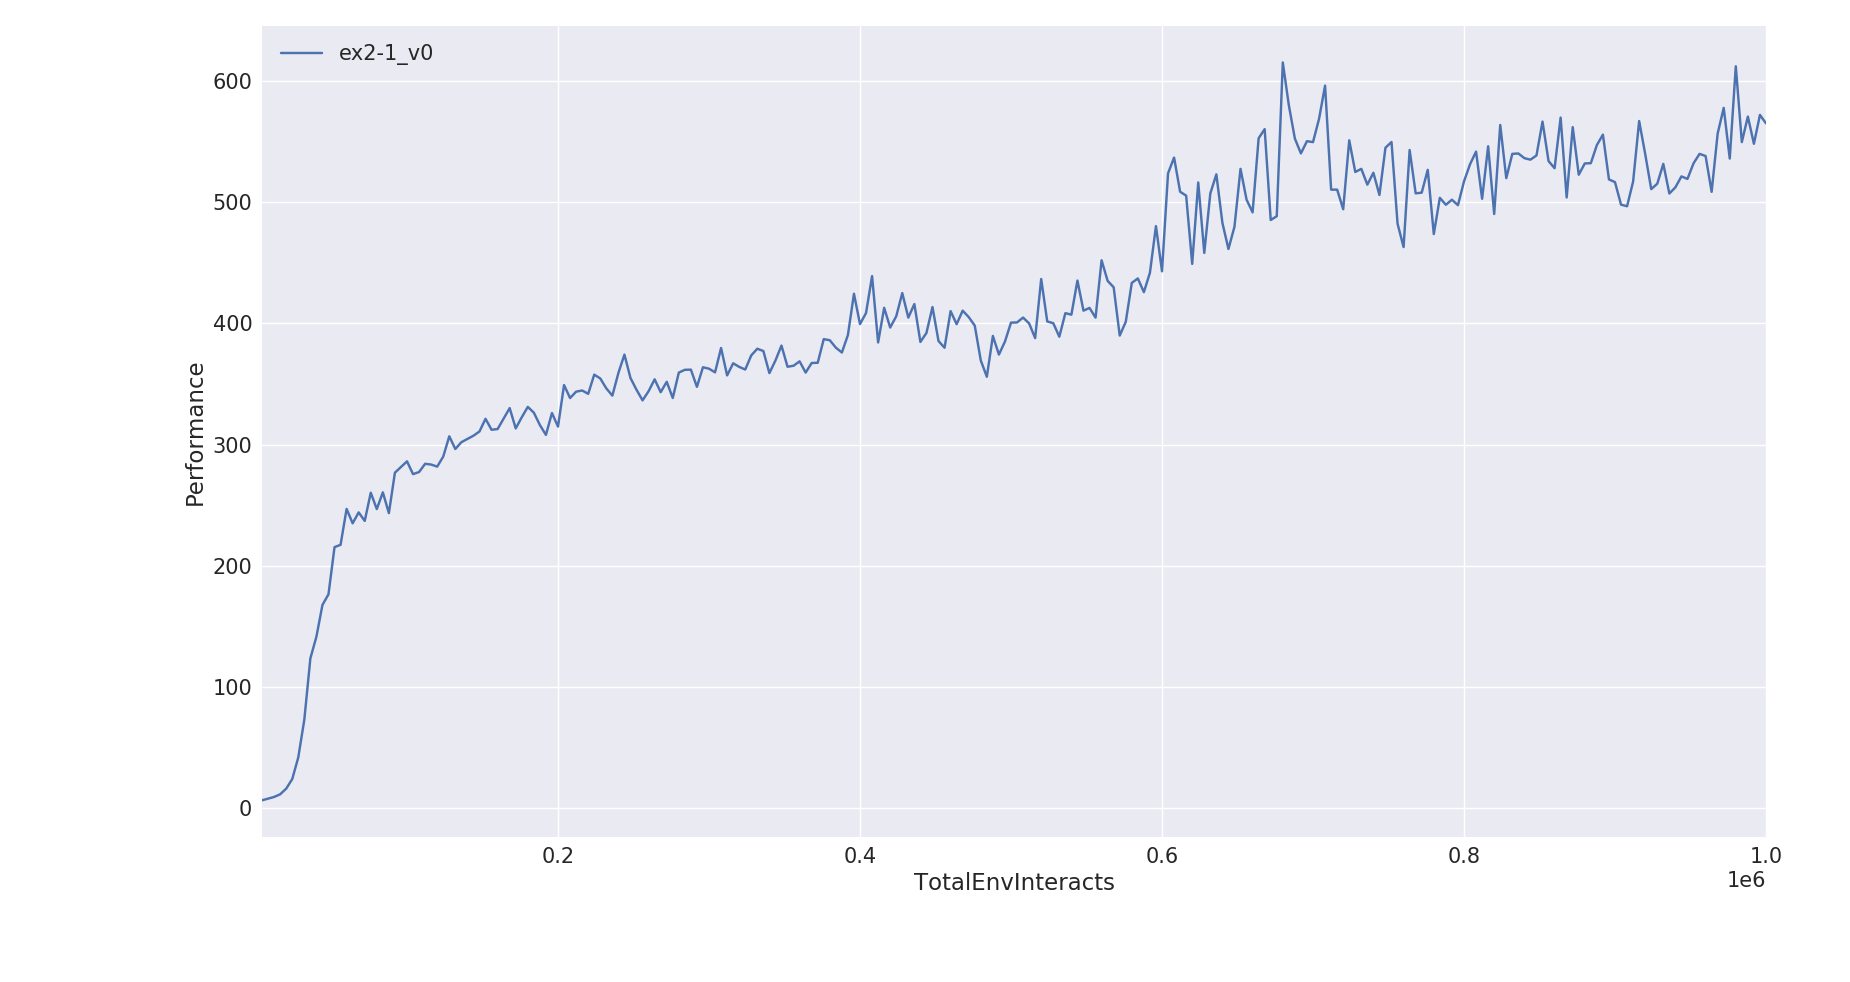
\includegraphics[width=0.32\textwidth]{../Img/spinningup_exercises/2_1/2_1_curve_v0_s10.png}
        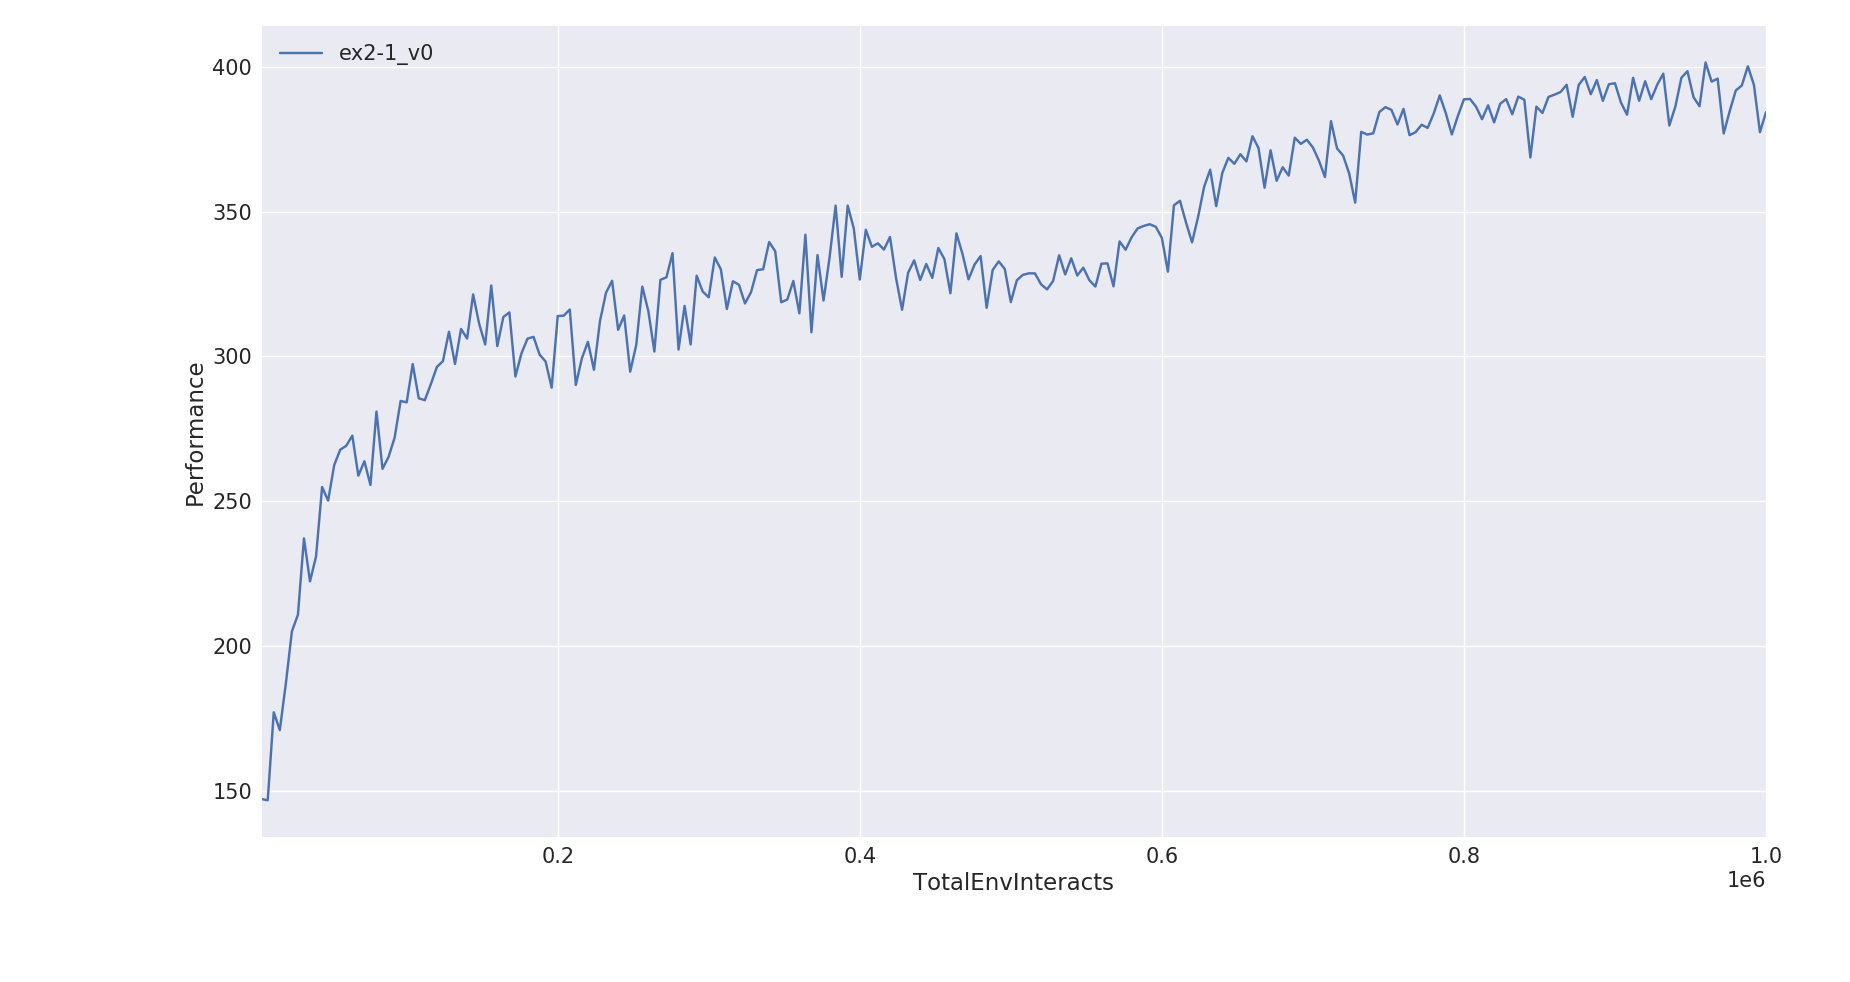
\includegraphics[width=0.32\textwidth]{../Img/spinningup_exercises/2_1/2_1_curve_v0_s20.png}
    \end{figure}

    The curve of v80 with different seeds are as follows:
    \begin{figure}[H]
        \centering
        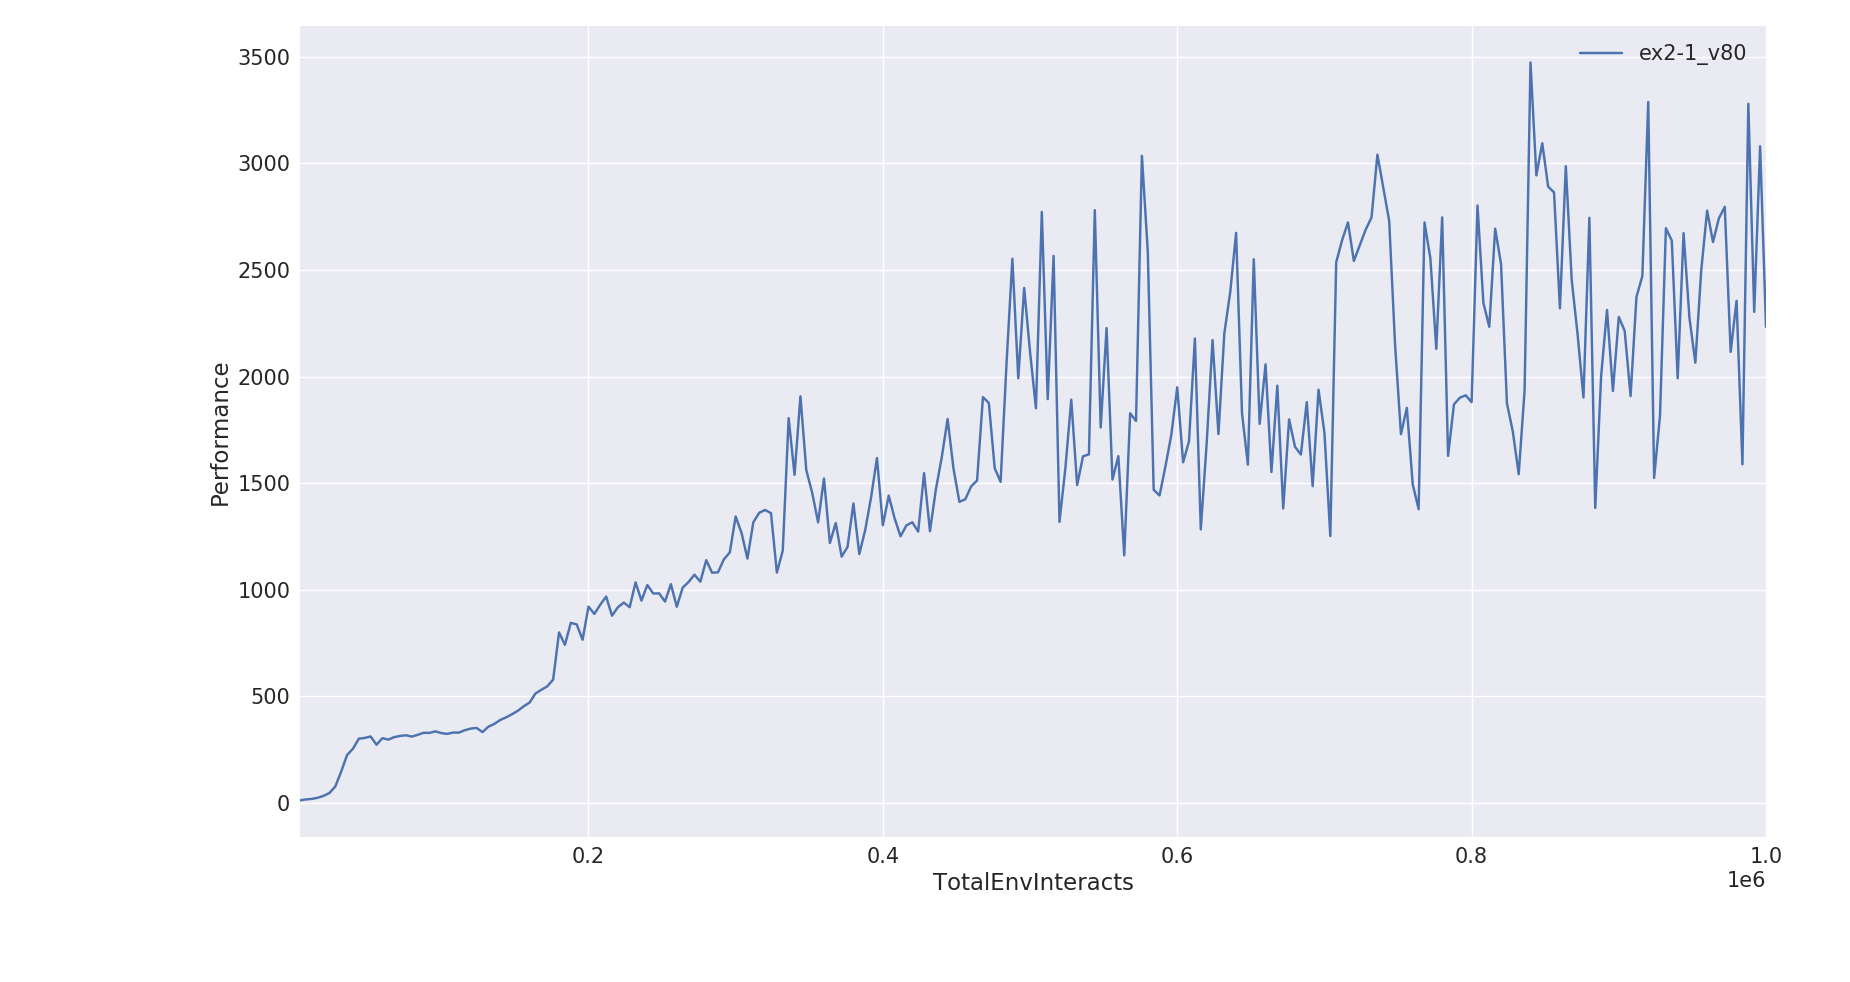
\includegraphics[width=0.32\textwidth]{../Img/spinningup_exercises/2_1/2_1_curve_v80_s0.png}
        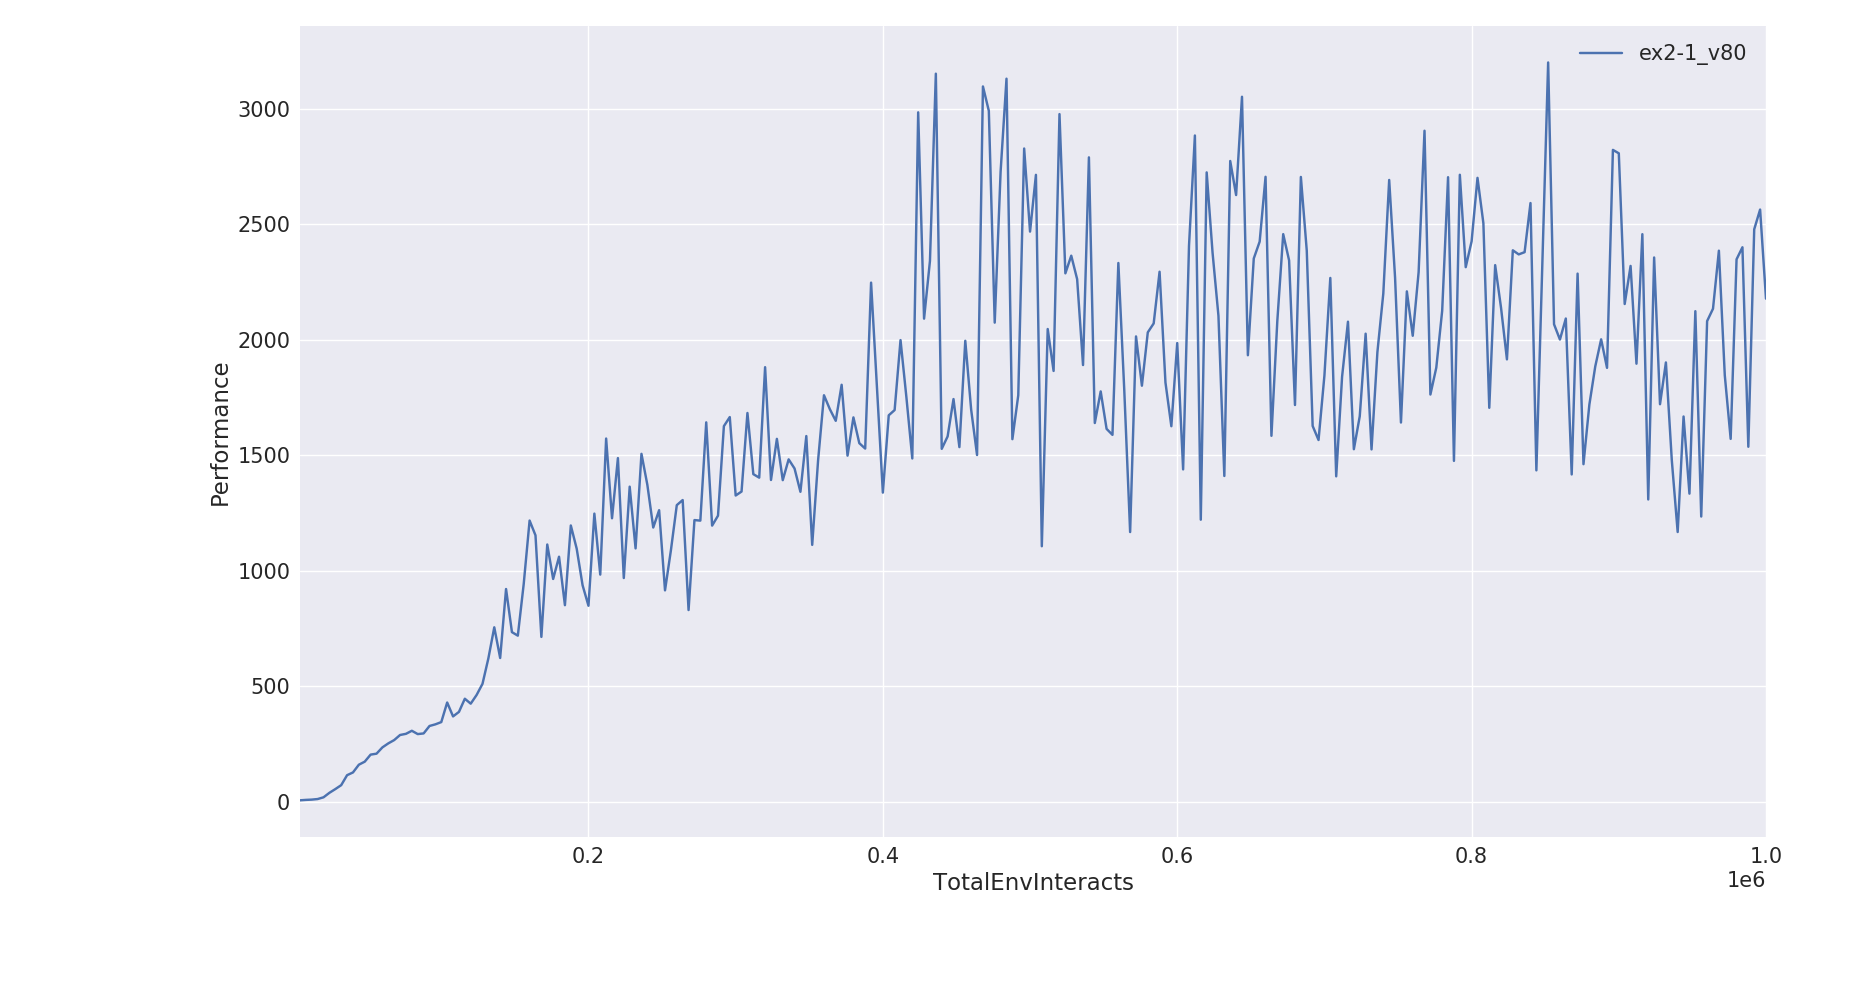
\includegraphics[width=0.32\textwidth]{../Img/spinningup_exercises/2_1/2_1_curve_v80_s10.png}
        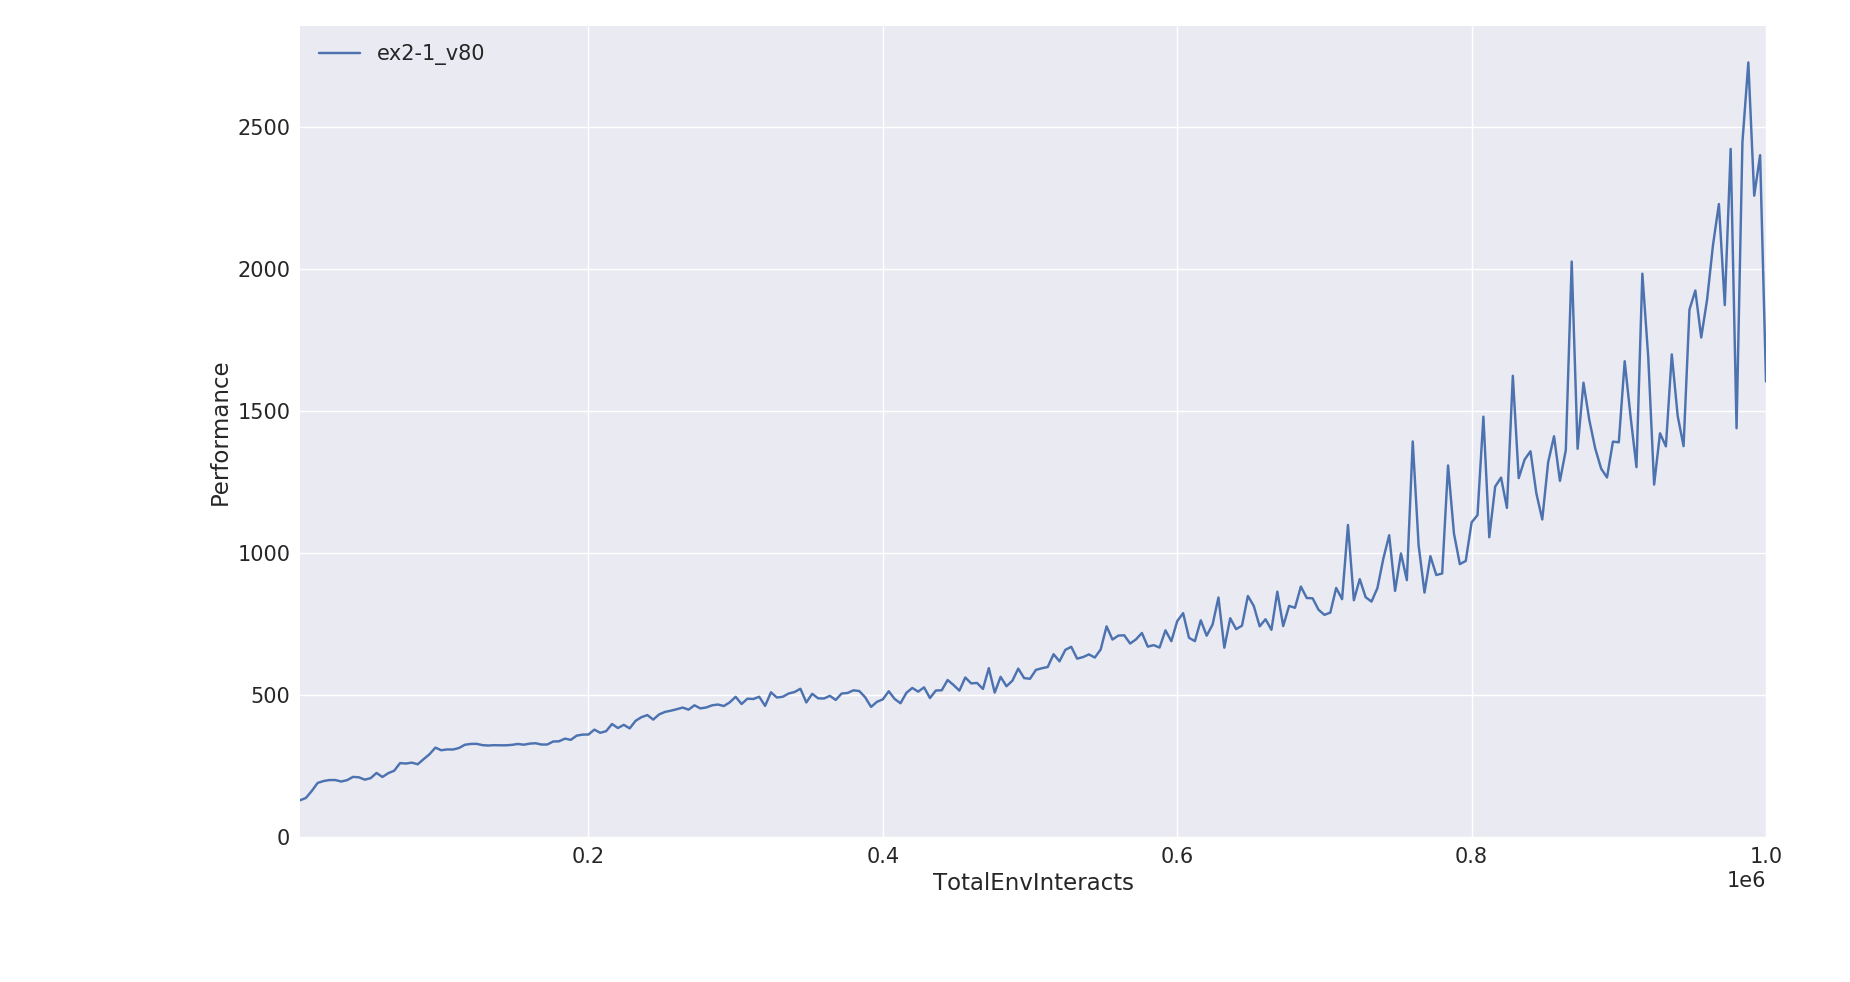
\includegraphics[width=0.32\textwidth]{../Img/spinningup_exercises/2_1/2_1_curve_v80_s20.png}
    \end{figure}

    The comparison between curve of v0 and v80, and their average and variance are as follows:
    \begin{figure}[H]
        \centering
        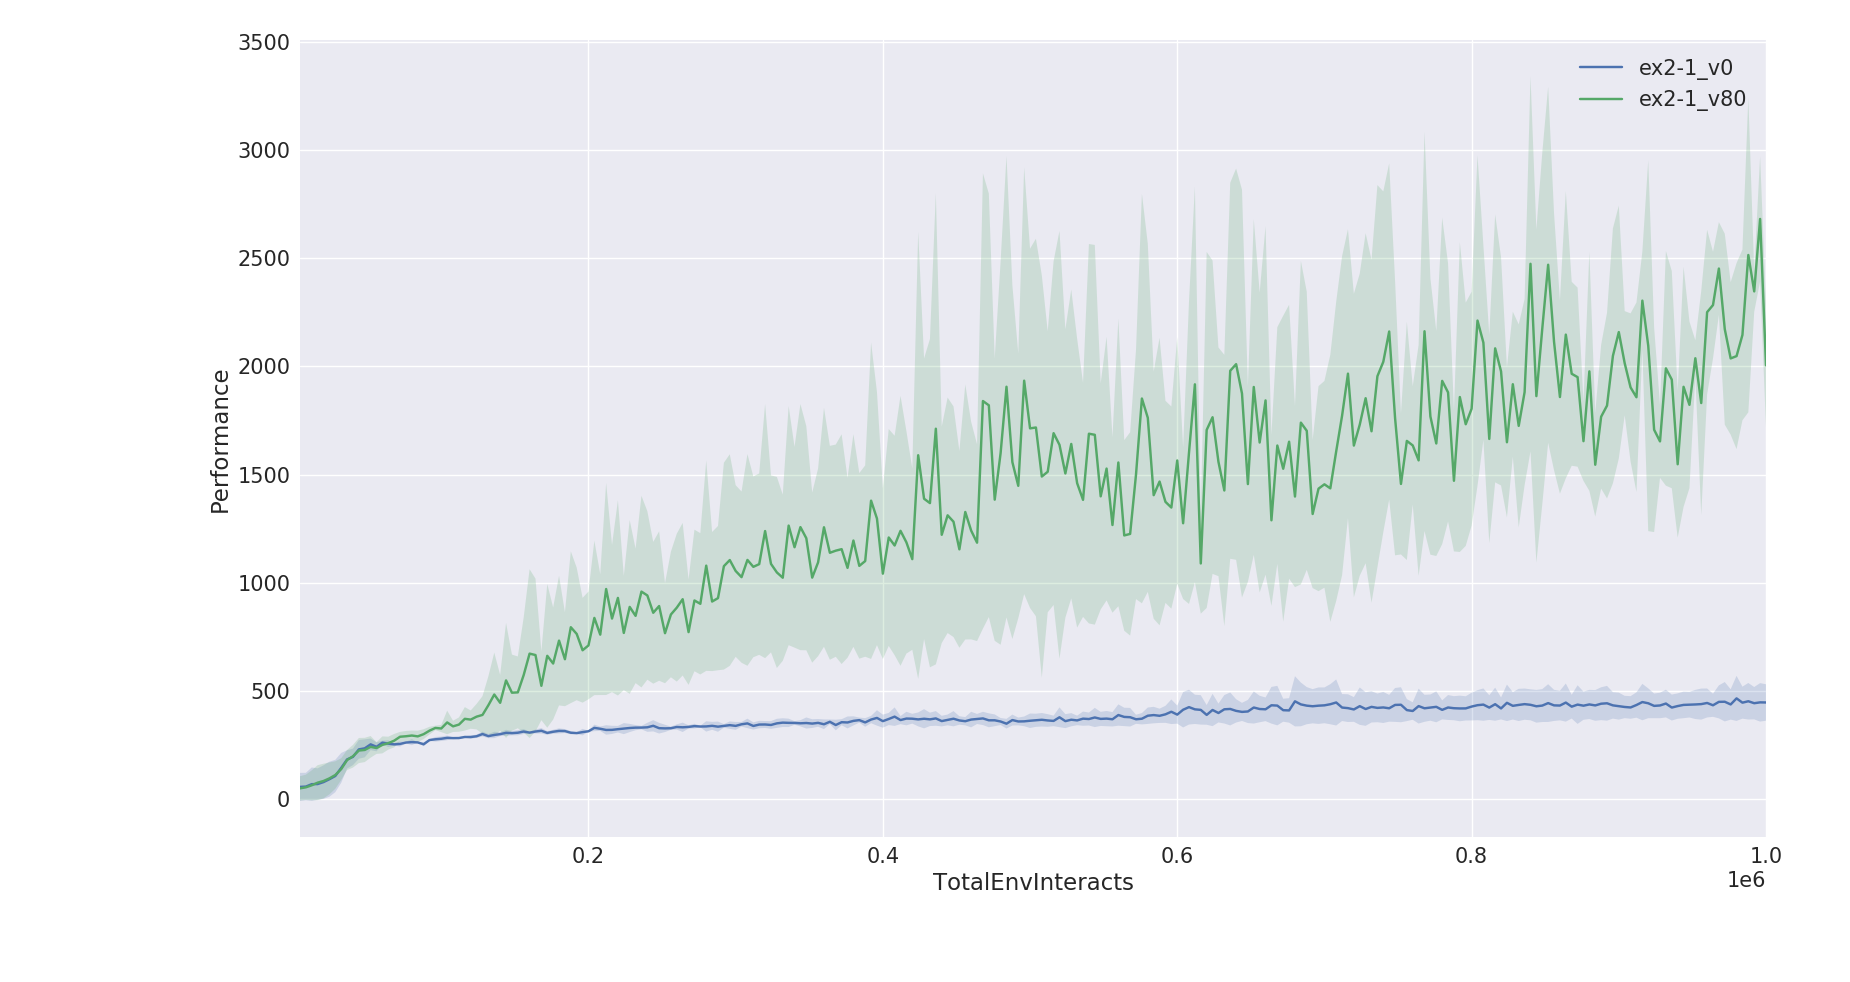
\includegraphics[width=\textwidth]{../Img/spinningup_exercises/2_1/2_1_curve_all.png}
    \end{figure}

    \item exercise 2\_2:
    The curve of the code without bug and with different seeds are as follows:
    \begin{figure}[H]
        \centering
        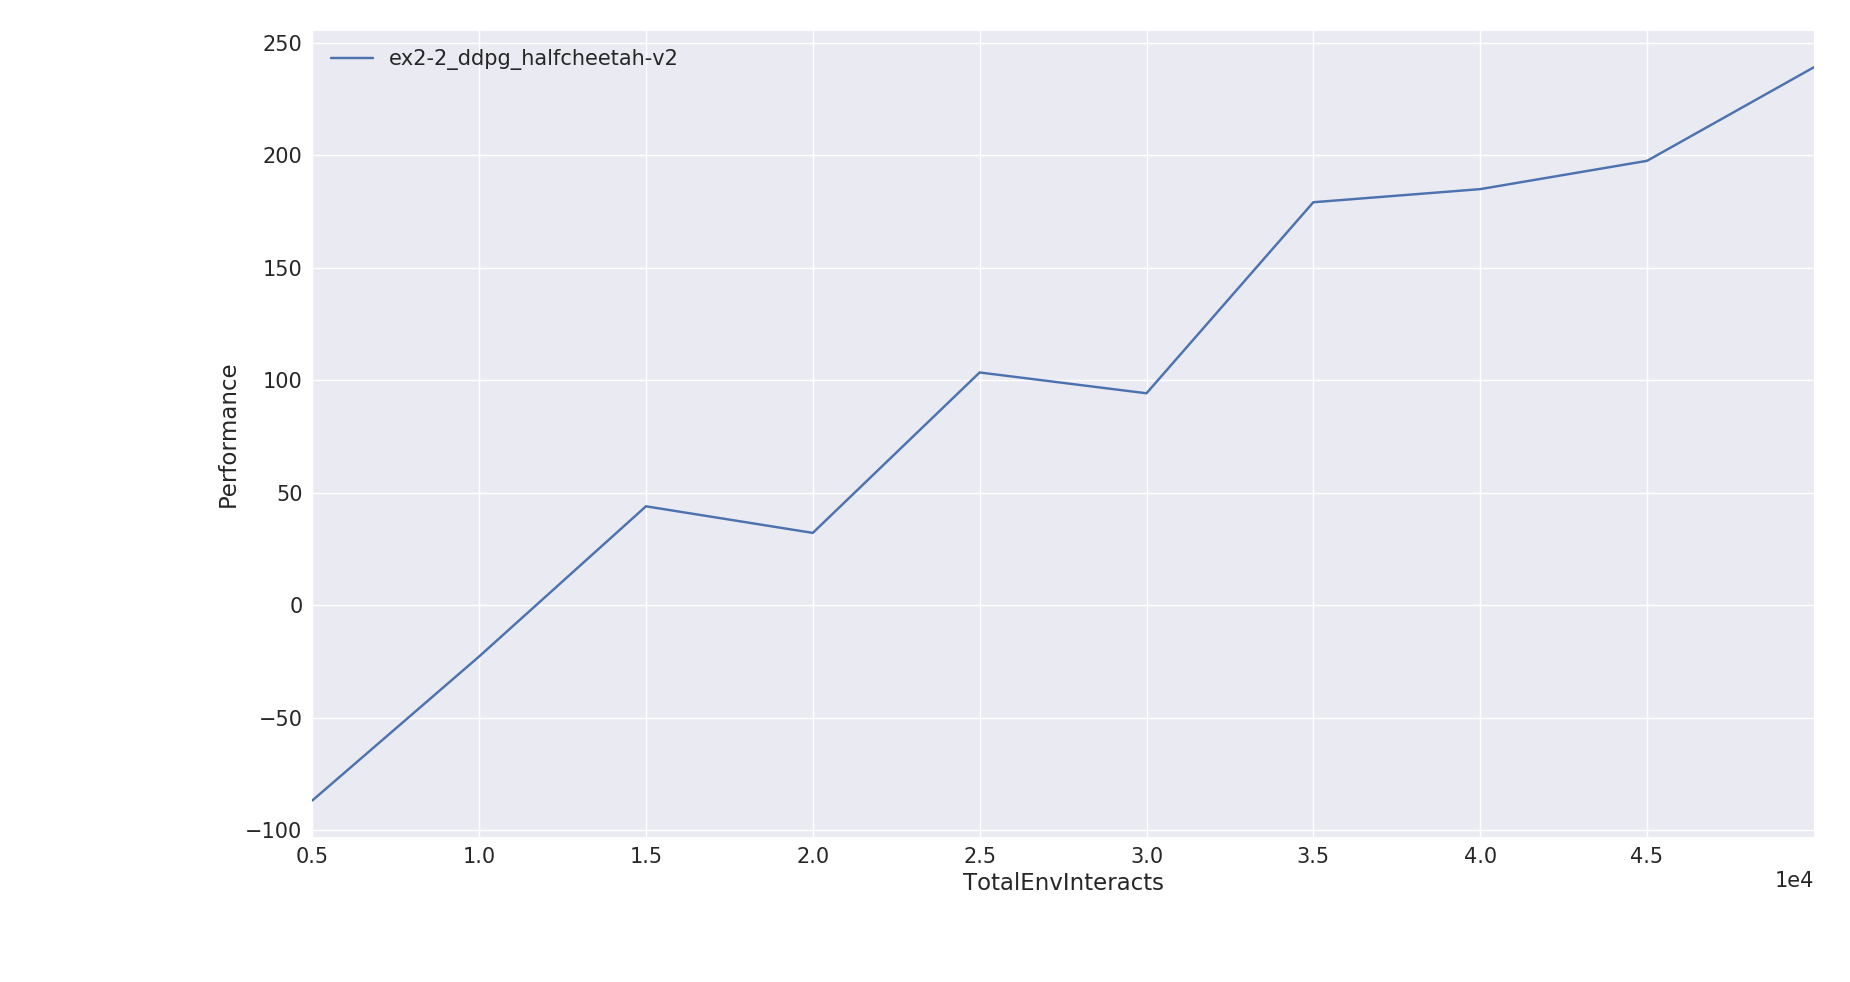
\includegraphics[width=0.32\textwidth]{../Img/spinningup_exercises/2_2/2_2_curve_s0.png}
        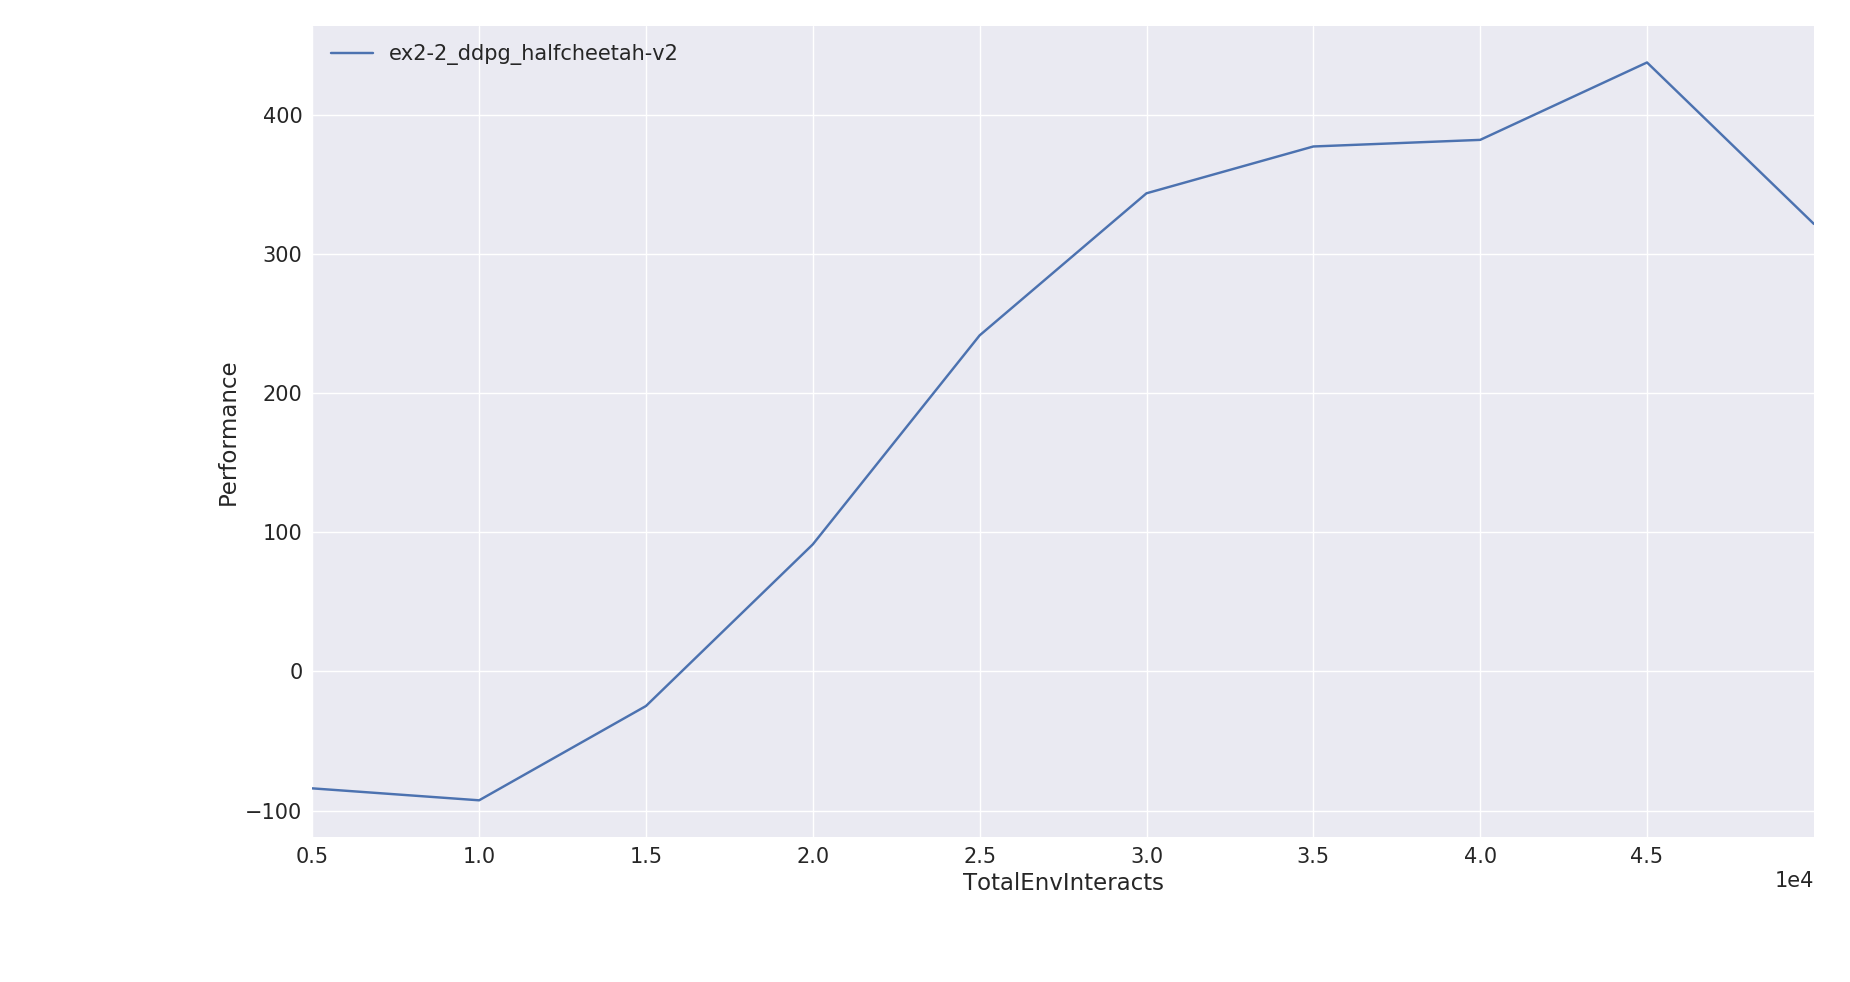
\includegraphics[width=0.32\textwidth]{../Img/spinningup_exercises/2_2/2_2_curve_s10.png}
        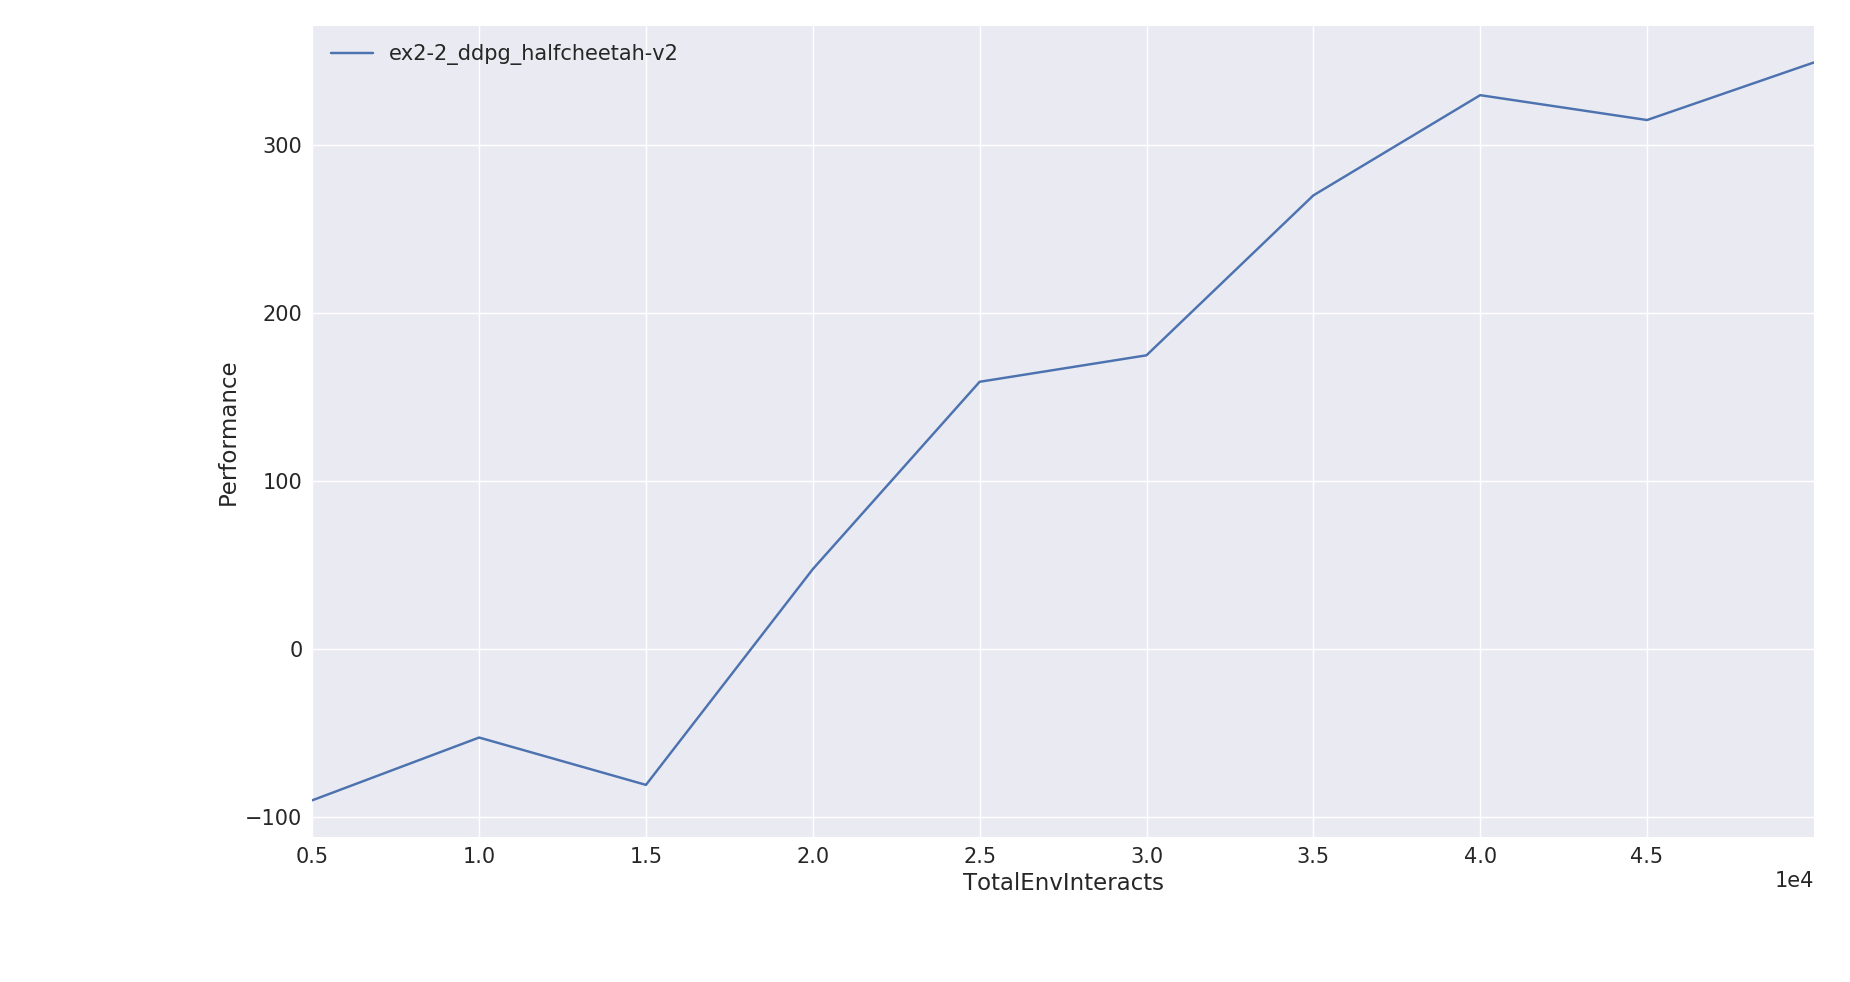
\includegraphics[width=0.32\textwidth]{../Img/spinningup_exercises/2_2/2_2_curve_s20.png}
    \end{figure}

    The curve of the code with bug and with different seeds are as follows:
    \begin{figure}[H]
        \centering
        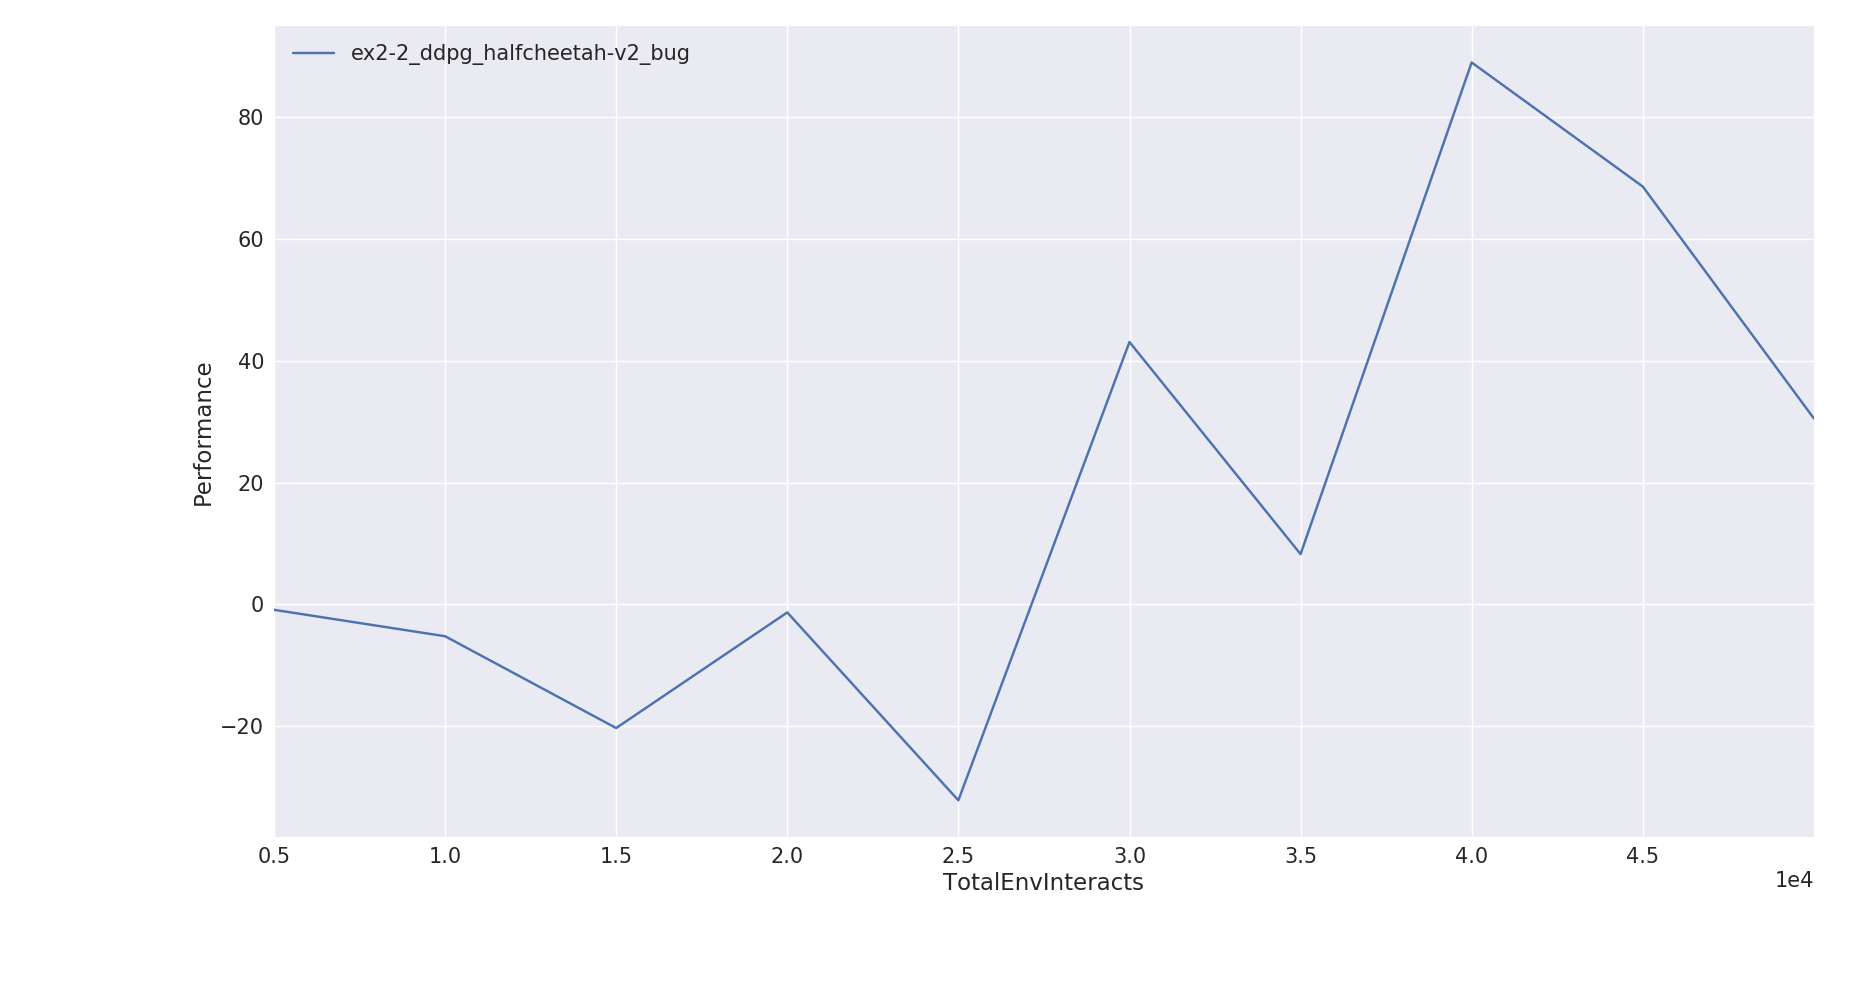
\includegraphics[width=0.32\textwidth]{../Img/spinningup_exercises/2_2/2_2_bug_curve_s0.png}
        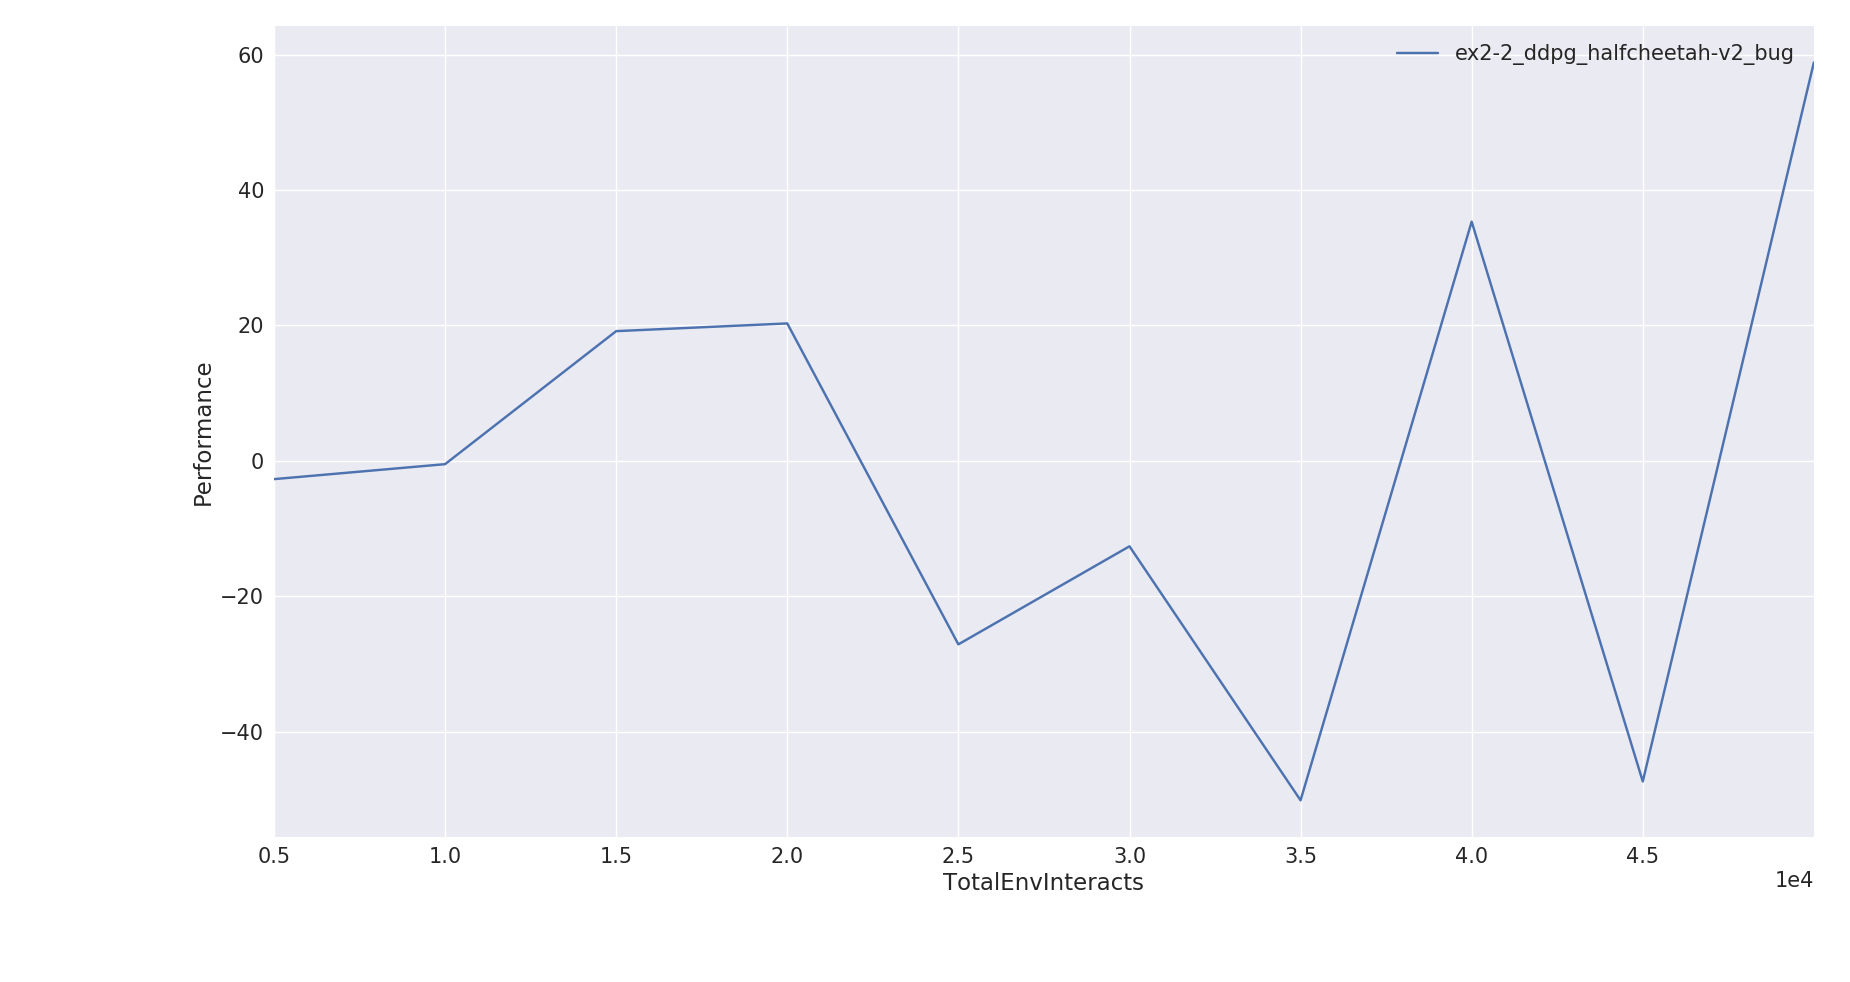
\includegraphics[width=0.32\textwidth]{../Img/spinningup_exercises/2_2/2_2_bug_curve_s10.png}
        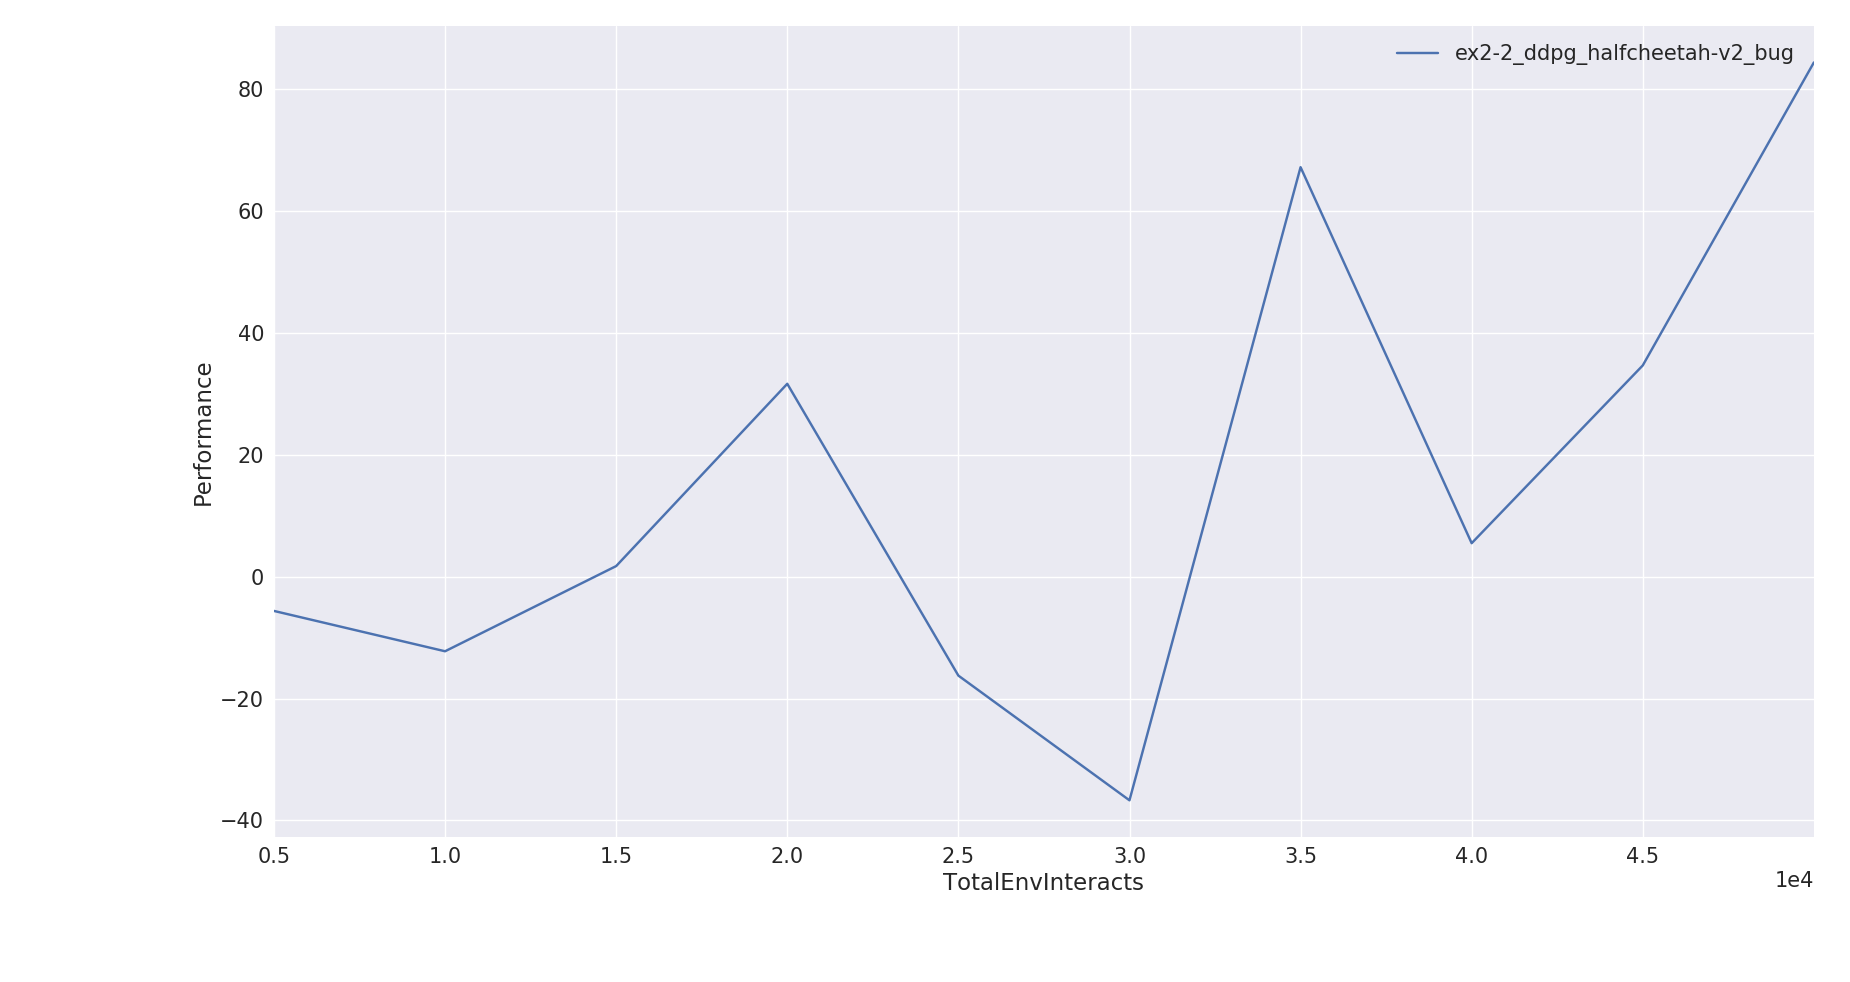
\includegraphics[width=0.32\textwidth]{../Img/spinningup_exercises/2_2/2_2_bug_curve_s20.png}
    \end{figure}

    The comparison between curve with and without bug, and their average and variance are as follows:
    \begin{figure}[H]
        \centering
        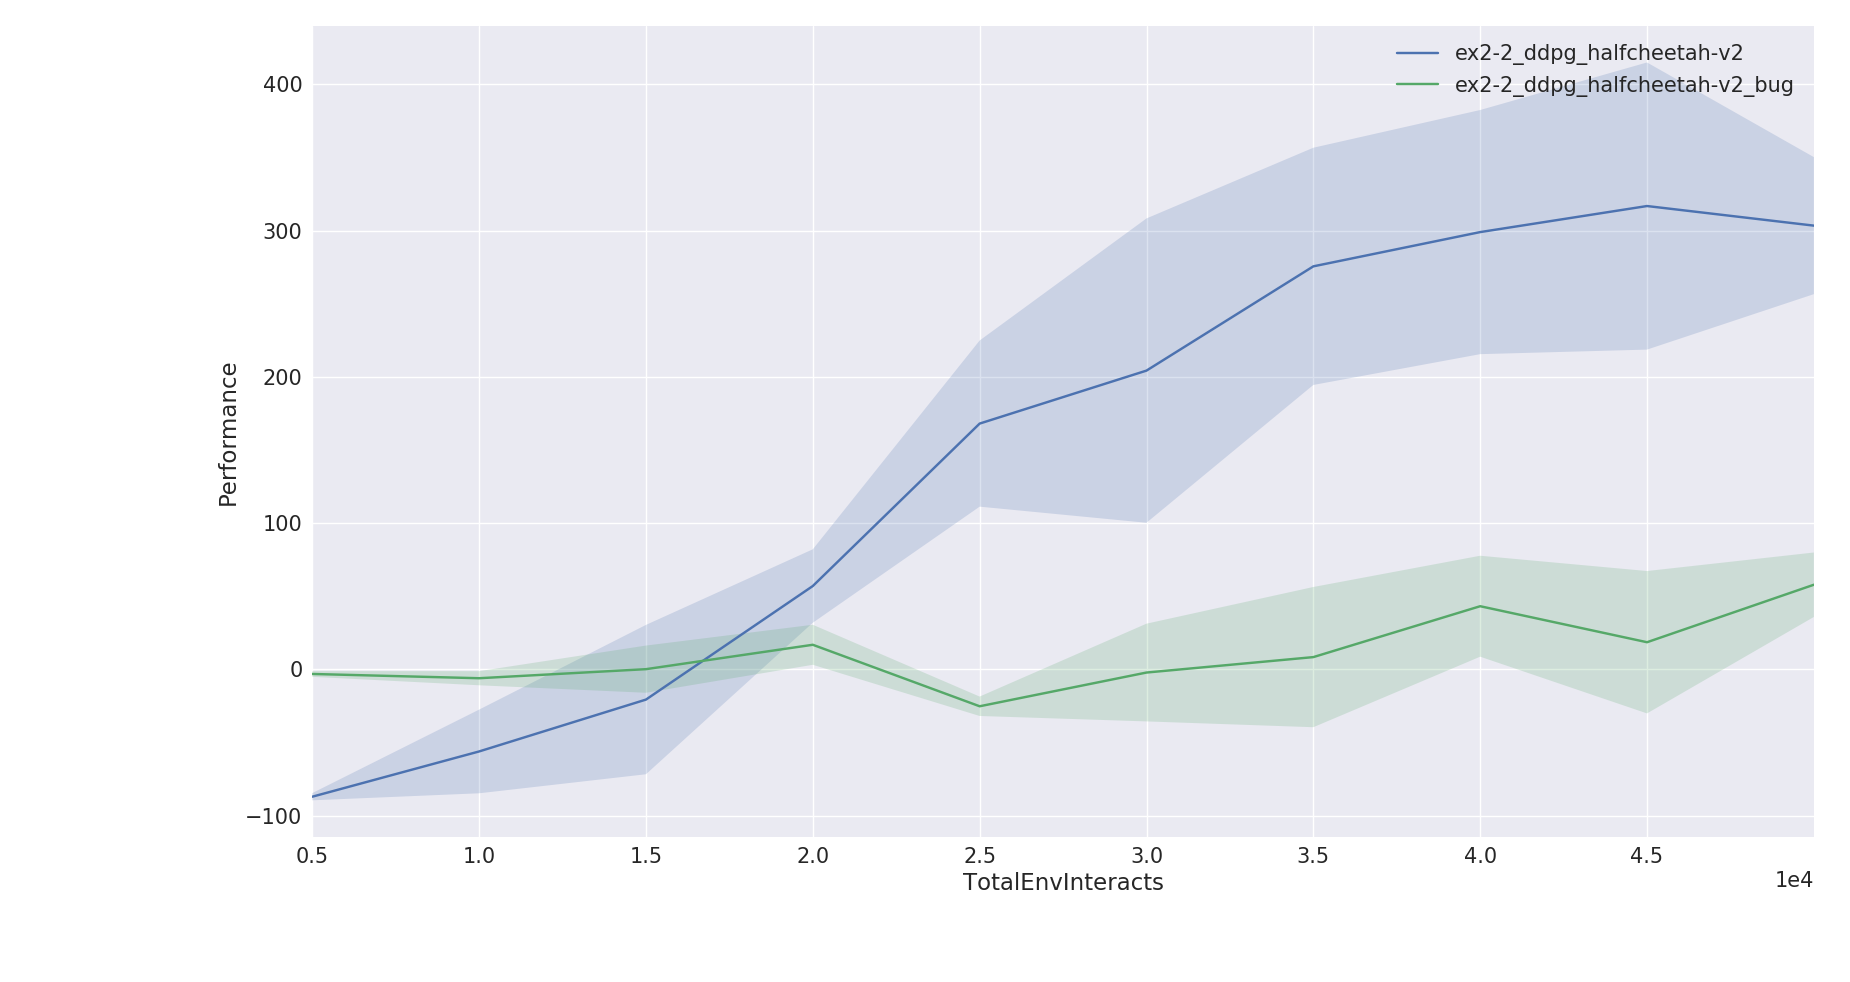
\includegraphics[width=\textwidth]{../Img/spinningup_exercises/2_2/2_2_curve_all.png}
    \end{figure}

    The code's bug is shown in the following figure:
    \begin{figure}[H]
        \centering
        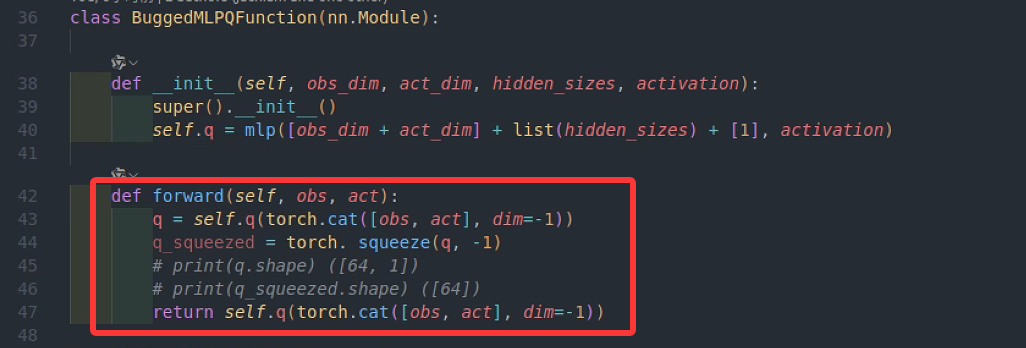
\includegraphics[width=\textwidth]{../Img/spinningup_exercises/2_2/2_2_mistake.png}
    \end{figure}


\end{itemize}



\end{homeworkProblem}

\newpage
\section{Part II: Performance Evaluation of Classical Bandit Algorithms}
You are required to use the Jupyter Notebook (Formerly known as the IPython Notebook) to submit your work.

\begin{itemize}
\item \textbf{Basic Setting} \\
We consider a time-slotted bandit system $(t=0,1,2, \ldots)$ with three arms. We denote the arm set as $\{1,2,3\}$. Pulling each arm $j(j \in\{1,2,3\})$ will obtain a reward $r_j$, which satisfies a Bernoulli distribution with mean $\theta_j\left(\operatorname{Bern}\left(\theta_j\right)\right)$, i.e.,
$$r_j= \begin{cases}1, & \text { w.p. } \theta_j \\ 0, & \text { w.p. } 1-\theta_j\end{cases}$$
where $\theta_j$ are parameters within $(0,1)$ for $j \in\{1,2,3\}$.

Now we run this bandit system for $N(N\gg 3)$ time slots. At each time slot $t$, we choose one and only one arm from these three arms, which we denote as $I(t) \in\{1,2,3\}$. Then we pull the arm $I(t)$ and obtain a reward $r_{I(t)}$. Our objective is to find an optimal policy to choose an arm $I(t)$ at each time slot $t$ such that the expectation of the aggregated reward is maximized, i.e.,
$$\max_{I(t), t=1, \ldots N} \mathbb{E}\left[\sum_{t=1}^N r_{r(t)}\right]$$
If we know the values of $\theta_j, j \in\{1,2,3\}$, this problem is trivial. Since $r_{T(t)} \sim \operatorname{Bern}\left(\theta_{I(t)}\right)$,
$$\mathbb{E}\left[\sum_{t=1}^N r_{I(t)}\right]=\sum_{t=1}^N \mathbb{E}\left[r_{I(t)}\right]=\sum_{t=1}^N \theta_{I(t)}$$
Let $I(t)=I^*=\underset{j \in\{1,2,3\}}{\arg \max } \theta_j$ for $t=1,2, \ldots, N$, then
$$\max _{I(t), t=1, \ldots, N} \mathbb{E}\left[\sum_{i=1}^N r_{I(t)}\right]=N \cdot \theta_{I^*}$$
However, in reality, we do not know the values of $\theta_j, j \in\{1,2,3\}$. We need to estimate the values $\theta_j$ via empirical samples, and then make the decisions at each time slot.
Next we introduce three classical bandit algorithms: $\epsilon$-greedy, UCB and Thompson sampling.

\item \textbf{Bandit Algorithms} \\
1. $\epsilon$-greedy Algorithm $(0 \leq \epsilon \leq 1)$
\begin{algorithm}[h]
\caption{$\epsilon$-greedy Algorithm}
\textbf{Initialize} $\hat{\theta}(j)\gets 0, \cnt(j)\gets 0, j \in \{1,2,3\}$
\begin{algorithmic}[1]
    \For {$t = 1,2,3,\ldots,N$}
        \State $I(t)\gets\begin{cases}
            \argmax\limits_{j\in\{1,2,3\}} \hat{\theta}_j, & \text{w.p. } 1-\epsilon \\
            \text{randomly choose from} \{1,2,3\}, & \text{w.p. } \epsilon
            \end{cases}$
        \State $\cnt(I(t))\gets \cnt(I(t)) + 1$
        \State $\hat{\theta}(I(t))\gets \hat{\theta}(I(t))+\frac{1}{\cnt(I(t))} \left[r_{I(t)}-\hat{\theta}(I(t))\right]$
    \EndFor
\end{algorithmic}
\end{algorithm}

2. UCB (Upper Confidence Bound) Algorithm \\
\begin{algorithm}[h]
\caption{UCB Algorithm}
\textbf{Initialize} $\hat{\theta}(j)\gets 0, \cnt(j)\gets 0, j \in \{1,2,3\}$
\begin{algorithmic}[1]
    \For {$t = 1,2,3$}
        \State $I(t)\gets t$
        \State $\cnt(I(t))\gets 1$
        \State $\hat{\theta}(I(t))\gets r_{I(t)}$
    \EndFor

    \For {$t = 4,\ldots,N$}
        \State $I(t)\gets\argmax\limits_{j\in\{1,2,3\}} \left(\hat{\theta}(j)+c\cdot \sqrt{\dfrac{2\log(t)}{\cnt(j)}} \right)$
        \State $\cnt(I(t))\gets \cnt(I(t)) + 1$
        \State $\hat{\theta}(I(t))\gets \hat{\theta}(I(t))+\frac{1}{\cnt(I(t))} \left[r_{I(t)}-\hat{\theta}(I(t))\right]$
    \EndFor
\end{algorithmic}
\end{algorithm}
\textbf{Note}: $c$ is a positive constant with a default value of 1.

3. Thompson sampling (TS) Algorithm \\
Recall that $\theta_j, j\in\{1, 2, 3\}$, are unknown parameters over (0, 1). From the Bayesian perspective, we assume their priors are Beta distributions with given parameters $(\alpha_j, \beta_j)$.
\begin{algorithm}[h]
\caption{TS Algorithm}
\textbf{Initialize} Beta parameter $(\alpha_j,\beta_j), j \in \{1,2,3\}$
\begin{algorithmic}[1]
    \For {$t = 1,2,3,\ldots,N$}
        \State \# Sample method
        \For {$j \in \{1,2,3\}$}
            \State Sample $\hat{\theta}(j) \sim \text{Beta}(\alpha_j, \beta_j)$
        \EndFor
        \State \# Select and pull the arm
        \State $I(t)\gets\argmax\limits_{j\in\{1,2,3\}} \hat{\theta}(j)$
        \State \# Update the distribution
        \State $\alpha_{I(t)}\gets \alpha_{I(t)} + r_{I(t)}$
        \State $\beta_{I(t)}\gets \beta_{I(t)} + 1 - r_{I(t)}$
    \EndFor
\end{algorithmic}
\end{algorithm}

\item \textbf{Simulation} \\
(1) Now suppose we obtain the Bernoulli distribution parameters from an oracle, which are shown in the following table below. Choose $N=10000$ and compute the theoretically maximized expectation of aggregate rewards over $N$ time slots. We call it the oracle value. Note that these parameters $\theta_j, j=1,2,3$ and oracle values are unknown to all bandit algorithms.
\begin{center}
\begin{tabular}{|c|c|c|c|}
    \hline $\operatorname{Arm} j$ & 1 & 2 & 3 \\
    \hline$\theta_j$ & 0.9 & 0.8 & 0.7 \\
    \hline
\end{tabular}
\end{center}

(2) Implement classical bandit algorithms with following settings: \\
- $N=5000$ \\
- $\epsilon$-greedy with $\epsilon=0.1,0.5,0.9$. \\
- UCB with $c=1,5,10$. \\
- Thompson Sampling with \\
$\left\{\left(\alpha_1, \beta_1\right)=(1,1),\left(\alpha_2, \beta_2\right)=(1,1),\left(\alpha_3, \beta_3\right)=(1,1)\right\}$ and \\
$\left\{\left(\alpha_1, \beta_1\right)=(601,401),\left(\alpha_2, \beta_2\right)=(401,601),\left(\alpha_3, \beta_3\right)=(2,3)\right\}$ \\
- Gradient bandit with baseline $b=0,0.8,5,20$. \\
- Parameterized gradient bandit with constant parameter $\beta=0.2,1,2,5$ \\
- Parameterized gradient bandit with time-varying parameters (you need to design a time-varying rule)

(3) Each experiment lasts for $N=5000$ turns, and we rum each experiment 1000 times. Results are averaged over these 1000 independent rums.

(4) Please report three performance metrics \\
- The total regret accumulated over the experiment. \\
- The regret as a function of time. \\
- The percentage of plays in which the optimal arm is pulled.

(5) Compute the gaps between the algorithm outputs and the oracle value. Compare the numerical results of $\epsilon$-greedy, UCB, Thompson Sampling and gradient bandit. Which one is the best? Then discuss the impacts of $\epsilon, C$, and $\alpha_j, \beta_j, b$, and $\beta$ respectively.

(6) What is the role of baseline in gradient bandit algorithm? Show your answer with simulation result.

(7) Give your understanding of the exploration-exploitation trade-off in bandit algorithms.

(8) Give your understanding of the adoption of sublinear regret as the performance threshold between good bandit algorithms and bad bandit algorithms.

\end{itemize}

\solution

(1) Since each arm's parameter is oracled, so we just need to choose the arm with the largest parameter to have the maximum expectation of aggregate rewards over $N$ time slots.

Since $\theta_1 = 0.9, \theta_2 = 0.8, \theta_3 = 0.7$, so we choose arm 1 everytime.

i.e.
\begin{align*}
\forall t, I(t)=I^* &= \argmax\limits_{j\in\{1,2,3\}}\theta_j=1 \\
\hat{\theta}_{I(t)} &= \theta_1 = 0.9 \\
r_{I(t)} \sim \text{Bern}(\theta_{I(t)}) &\Rightarrow \mathbb{E}(r_{I(t)}) = \hat{\theta}_{I(t)}
\end{align*}
So the maximum expected value is
\begin{align*}
&\quad\ \max_{I(t),t=1,2,\cdots,N}\ \mathbb{E}\left[\sum_{t=1}^Nr_{I(t)}\right] \\
&= \max_{I(t),t=1,2,\cdots,N}\ \sum_{t=1}^N\mathbb{E}\left[r_{I(t)}\right] \\
&= N \cdot \hat{\theta}_{I(t)} \\&= 10000 \times 0.9 \\
&= 9000
\end{align*}
So above all, with the given oracle parameters, the maximum expected value is 9000.

(2), (3) The implementation codes are in the `hw4\_code.ipynb' file.

(4) 1. The epsilon-greedy algorithm
\begin{table}[h]
    \centering
    \begin{tabular}{c c c}
    \toprule
    parameter & Average Regret & Optimal Percentage \\
    \midrule
    $\epsilon=0.1$ & 54.35  & 92.48\% \\
    $\epsilon=0.5$ & 251.34 & 66.30\% \\
    $\epsilon=0.9$ & 449.43 & 39.95\% \\
    \bottomrule
\end{tabular}
\vspace{-0.5cm}
\end{table}

\newpage
The regret and optimal percentage for $\epsilon$-greedy algorithm as a function of time are shown in the following figures:
\begin{figure}[h]
    \centering
    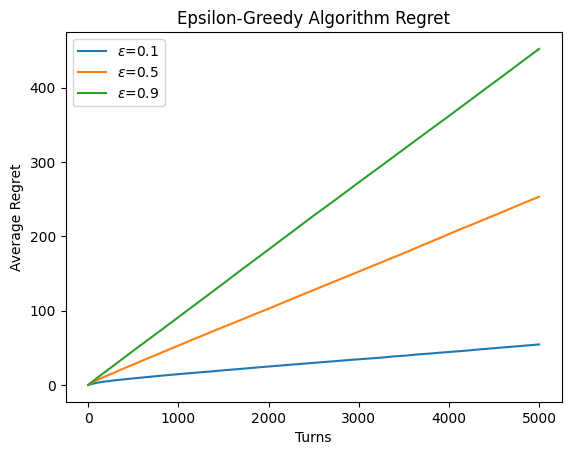
\includegraphics[width=0.49\textwidth]{./figure/epsilon_greedy_regret.png}
    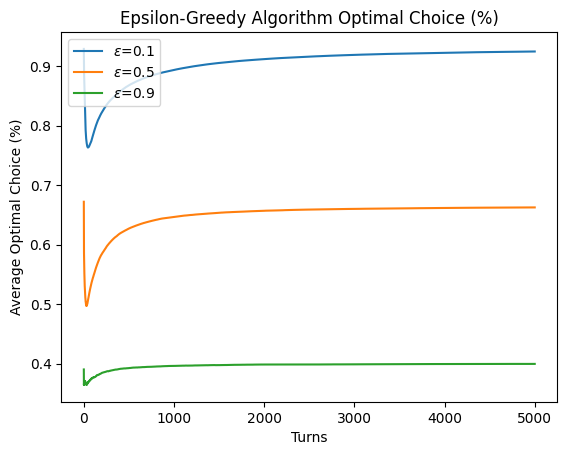
\includegraphics[width=0.49\textwidth]{./figure/epsilon_greedy_optimal.png}
\end{figure}

2. The UCB algorithm
\begin{table}[h]
    \centering
    \begin{tabular}{c c c}
    \toprule
    parameter & Average Regret & Optimal Percentage \\
    \midrule
    $c=1$  & 112.75 & 82.51\% \\
    $c=5$  & 372.65 & 47.20\% \\
    $c=10$ & 436.05 & 40.18\% \\
    \bottomrule
\end{tabular}
\end{table}

The regret and optimal percentage for UCB algorithm as a function of time are shown in the following figures:
\begin{figure}[h]
    \centering
    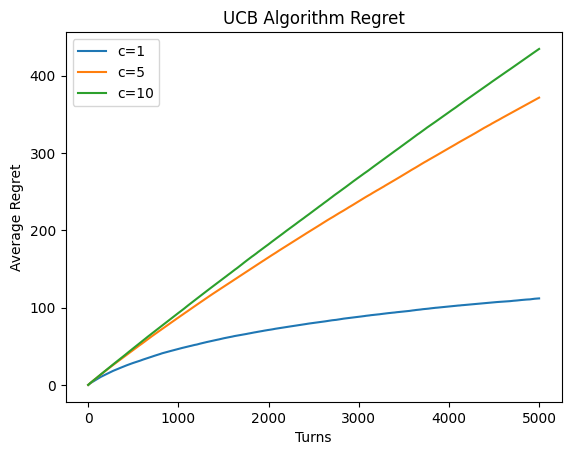
\includegraphics[width=0.49\textwidth]{./figure/UCB_regret.png}
    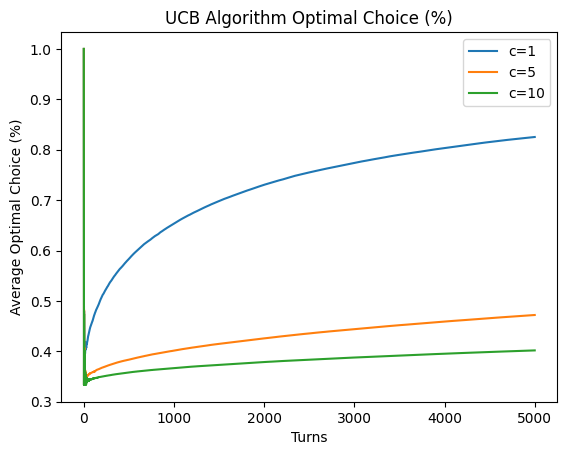
\includegraphics[width=0.49\textwidth]{./figure/UCB_optimal.png}
\end{figure}


3. The Thompson Sampling algorithm
\begin{table}[!htbp]
    \centering
    \begin{tabular}{c c c}
    \toprule
    parameter & Average Regret & Optimal Percentage \\
    \midrule
    $\alpha,\beta=[(1,1),(1,1),(1,1)]$         & 14.36  & 97.58\% \\
    $\alpha,\beta=[(601,401),(401,601),(2,3)]$ & 708.15 & 29.07\% \\
    \bottomrule
\end{tabular}
\end{table}

\newpage
\begin{figure}[h]
    \centering
    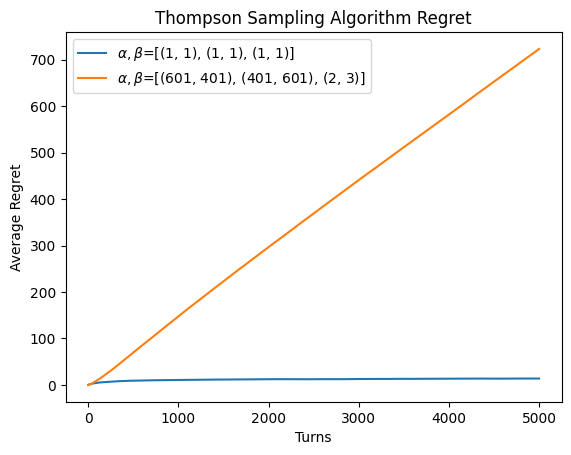
\includegraphics[width=0.49\textwidth]{./figure/TS_regret.png}
    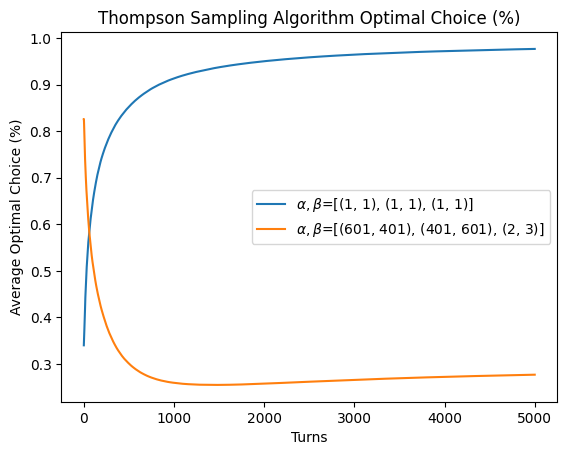
\includegraphics[width=0.49\textwidth]{./figure/TS_optimal.png}
\end{figure}

4. The Gradient Bandit algorithm \\
The step size is set to be $\alpha=0.1$. For the time-varient case, to have a smooth varying, set $\beta_0=0.1, \beta_T=10$:
$$\beta(t) = \beta_0 + \left( \frac{\log\left(1 + 9 \cdot \frac{t}{T} \right)}{\log(10)} \right) \cdot (\beta_T - \beta_0) = 0.1 + \left( \frac{\log\left(1 + 9 \cdot \frac{t}{T} \right)}{\log(10)} \right) \cdot (10 - 0.1)$$
And the baseline is set to be $B_t=\bar{R}_t$ is $b=-1$, otherwise it is set to be $B_t=b$.
\begin{table}[h]
    \centering
    \begin{tabular}{c c c}
    \toprule
    parameter & Average Regret & Optimal Percentage \\
    \midrule
    $b=0$   & 71.36  & 88.72\% \\
    $b=0.8$ & 50.37  & 92.72\% \\
    $b=5$   & 381.22 & 44.73\% \\
    $b=20$  & 490.65 & 33.18\% \\
    \midrule
    $\beta=0.2$ & 176.42 & 74.77\% \\
    $\beta=1$   & 49.97  & 92.60\% \\
    $\beta=2$   & 30.06  & 95.67\% \\
    $\beta=5$   & 16.57  & 97.55\% \\
    \midrule
    time-varying & 19.22 & 97.22\% \\
    \bottomrule
\end{tabular}
\vspace{-0.5cm}
\end{table}

\begin{figure}[!htbp]
    \centering
    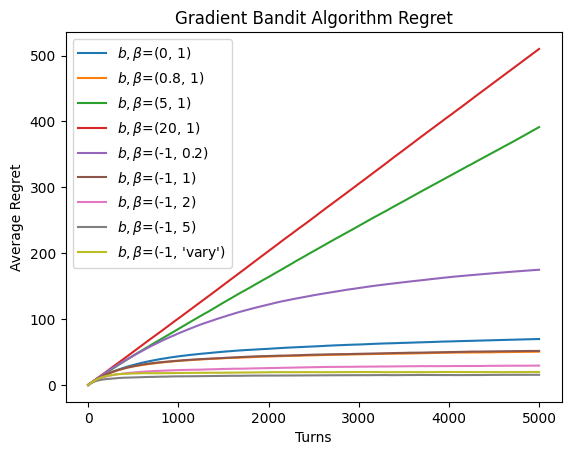
\includegraphics[width=0.49\textwidth]{./figure/gradient_bandit_regret.png}
    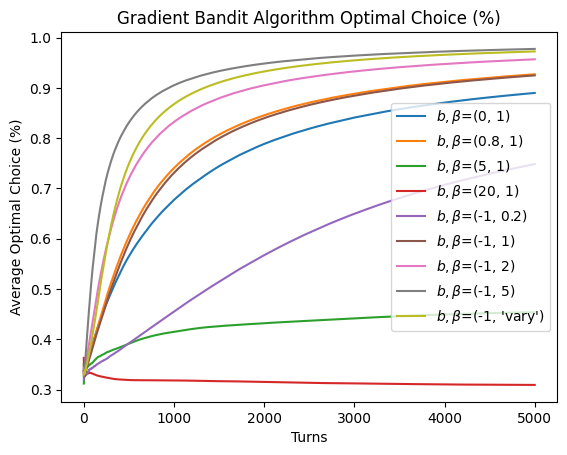
\includegraphics[width=0.49\textwidth]{./figure/gradient_bandit_optimal.png}
\end{figure}
\newpage

(5) The gap's comparison between the algorithms with different parameters is as follows:
\begin{table}[!htbp]
    \centering
    \colorbox{orange}{best}\ \colorbox{cyan}{second best} \\
    \begin{tabular}{c|c|c}
    \toprule
    \textbf{Algorithm} & \textbf{Parameter} & \textbf{Gap} \\
    \midrule
    \multirow{3}{*}{\centering $\epsilon$-Greedy}   & $\epsilon=0.1$ & 54.35  \\
                                                    & $\epsilon=0.5$ & 251.34 \\
                                                    & $\epsilon=0.9$ & 449.43 \\
    \midrule
    \multirow{3}{*}{\centering UCB} & $c=1$  & 112.75 \\
                                    & $c=5$  & 372.65 \\
                                    & $c=10$ & 436.05 \\
    \midrule
    \multirow{2}{*}{\centering TS}  & $\alpha,\beta=[(1,1),(1,1),(1,1)]$         & \cellcolor{orange}{14.36}  \\
                                    & $\alpha,\beta=[(601,401),(401,601),(2,3)]$ & 708.15 \\
    \midrule
    \multirow{10}{*}{\centering Gradient}   & $b=0$   & 71.36  \\
                                            & $b=0.8$ & 50.37  \\
                                            & $b=5$   & 381.22 \\
                                            & $b=20$  & 490.65 \\
    \cline{2-3}
    & $\beta=0.2$ & 176.42 \\
    & $\beta=1$   & 49.97  \\
    & $\beta=2$   & 30.06  \\
    & $\beta=5$   & \cellcolor{cyan}{16.57} \\
    \cline{2-3}
    & time-varying & 19.22 \\
    \bottomrule
    \end{tabular}
\end{table}

Comparing all rewards among the experiments we have done, we could find that the Thompson Sampling algorithm with parameter $\alpha,\beta=[(1,1),(1,1),(1,1)]$ is the best one, and gradient bandit algorithm with parameter $\beta=5$ is the second best one.

Then we can discuss the impacts of $\epsilon$, $c$, and $\alpha_{j}$, $\beta_{j}$, $b$, $\beta$ respectively.
\begin{itemize}
\item $\epsilon$-greedy algorithm \\
We have a parameter $\epsilon$, in our experiments, lower $\epsilon$ has a lower regret, however, it is still linear to the time.

\item the UCB algorithm \\
We choose the arm by the metric $\hat{\theta}(j)+c\cdot \sqrt{\dfrac{2\log(t)}{\cnt(j)}}$. In our experiments, we could find that the regret of the UCB algorithm with $c=1$ is the lowest. And the regret is sublinear to the time. Larger $c$ has a higher regret, and the regret looks like linear to the time when $c=5,10$.

\item the Thompson Sampling algorithm \\
In the Beta-Bernoulli Thompson Sampling algorithm, we have a parameter $\alpha$ and $\beta$ to decide $\hat{\theta}_j$ as it $\sim \Beta(\alpha,\beta)$, in our experiences, we could discover that $\alpha,\beta=[(1,1),(1,1),(1,1)]$ is the best one. This is because the prior brief is closer to the true distribution of the reward, and it is not in a wrong direction. $\alpha,\beta=[(601,401),(401,601),(2,3)]$ could be regarded as doing some of the experiments, but the experiment is in a wrong distribution with the oracle distribution, so a worse prior lead to a worse performance.

\item the Gradient Bandit algorithm \\
The motivation of introducting baseline in the policy gradient algorithm is mainly used to reduce variance and accelerate convergence to make the algorithm more stable. The parameter $\beta$ adjust the weights for the perference of the arm.

In ours experiments, baseline $b=0.8$ have a better performance all $b$s. This is because $b=0.8$ is closer to the best arm's oracle distribution $\theta_1=0.9$, so it has a better performance. And larger $\beta$ means more important to the perference of the arm so $\beta=5$ has a better performance. And in theoretically, $\beta$ should be small at beginning for exploration, and be larger for exploitation latter. However, in our experiments, the time-varying $\beta$ is worse than $\beta=5$. This may because the time-varying function is not well selected.
\end{itemize}

(6) The baseline in the gradient bandit algorithm is a reference point for the reward. It is used to reduce the variance of the reward and make the algorithm more stable. We can test the performance of the gradient bandit algorithm with different baseline and different $\beta$. $b=-1$ representing the baseline is the average reward $\bar{R}_t$.

\begin{table}[h]
    \centering
    \colorbox{orange}{best}\ \colorbox{cyan}{second best} \\
    \begin{tabular}{c c c}
    \toprule
    parameter & Average Regret & Optimal Percentage \\
    \midrule
    $b=-1, \beta=1$ & 51.38 & 92.57\% \\
    $b=0,  \beta=1$ & 73.54 & 88.41\% \\
    $b=1,  \beta=1$ & 50.44 & 92.65\% \\
    \midrule
    $b=-1, \beta=2$ & 29.04 & 95.66\% \\
    $b=0,  \beta=2$ & 76.34 & 86.75\% \\
    $b=1,  \beta=2$ & 30.16 & 95.75\% \\
    \midrule
    $b=-1, \beta=5$ & \cellcolor{orange}{16.07}  & 97.57\% \\
    $b=0,  \beta=5$ & 150.11 & 73.57\% \\
    $b=1,  \beta=5$ & \cellcolor{cyan}{16.59}  & 97.33\% \\
    \bottomrule
\end{tabular}
\vspace{-0.5cm}
\end{table}

\begin{figure}[!htbp]
    \centering
    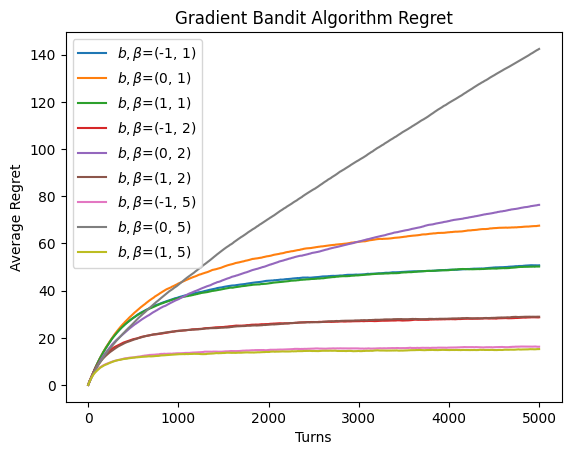
\includegraphics[width=0.49\textwidth]{./figure/gradient_bandit_baseline_regret.png}
    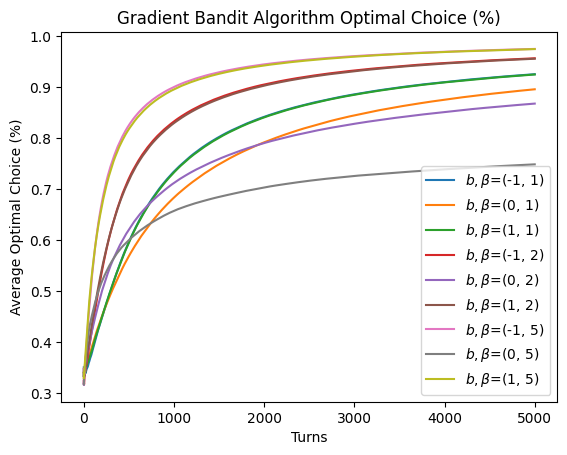
\includegraphics[width=0.49\textwidth]{./figure/gradient_bandit_baseline_optimal.png}
    \vspace{-0.5cm}
\end{figure}

And we can see that $\beta$ is the most significant parameter. Setting the baseline to be the average reward $\bar{R}_t$ has a better performance in ours experiments. If the baseline set not suitable, even a better $\beta$ could lead to a worse performance. For example, in ours experiment $b=0, \beta=5$ has a much larger average regret. And with baseline $B_t=\bar{R}_t, \beta=5$ has a much better performance. $b=0$ means without baseline, and we can see that in all settings of $\beta$, $b=0$, i.e. without baseline always has the highest regret.

(7) Exploration-Exploitation is a basic and popular topic in Reinforcement Learning. And it is also a very important topic in the bandit algorithm. At the beginning of playing with the bandit, we know nothing about the bandit. So we have to explore the bandit, gaining data from the previous decisions and feedbacks. Then after getting some information about the bandit, we can exploit them.

However, there must have a trade-off between exploration and exploitation. That is we have no idea how many times to explore, and when to start to exploit. If we always explore, we will never exploit to obtain better reward. And if we always exploit, we do not explore, and we may miss the best decision, go along the wrong way further and further. So we need to find a balance between exploration and exploitation. And this is the exploration-exploitation trade-off.
\begin{itemize}
\item $\epsilon$-greedy algorithm \\
We have a parameter $\epsilon$ to decide the probability of exploration and exploitation. If we set $\epsilon$ to be a small value, we will have a high probability to exploit the best arm we have found. And we will have a low probability to explore other arms. If we set $\epsilon$ to be a large value, we will have a high probability to explore other arms. And we will have a low probability to exploit the best arm we have found. So theoretically, the most suitable $\epsilon$ is time-varying: a larger value at the beginnig, and gradually decrease to a small value.

\item the UCB algorithm \\
We choose the arm by the metric $\hat{\theta}(j)+c\cdot \sqrt{\frac{2\log(t)}{\cnt(j)}}$. Where $\hat{\theta}(j)$ could be regard as exploitation, and $c\cdot \sqrt{\frac{2\log(t)}{\cnt(j)}}$ could be regard as exploration.

As for $c$, it is the parameter the decribe the degree of exploration. As $c$ increase, It turns to be more likely to explore. Correspondingly, as $c$ decrease, it more likely to exploitation.

So theoretically, the most suitable $c$ is time-varying: a larger value at the beginnig, and gradually decrease to a small value.

\item the Thompson Sampling algorithm \\
In the Beta-Bernoulli Thompson Sampling algorithm, we have a parameter $\alpha$ and $\beta$ to decide $\hat{\theta}_j\sim \Beta(\alpha,\beta)$. The Thompson Sampling algorithm is somehow more like a Bayesian method. We have a prior belief of the distribution of the reward. And we update the belief according to the reward we get.

The initial parameters $\alpha$ and $\beta$ are the prior belief of the distribution of the reward. And we update the parameters according to the reward we get with the Beta-Binomial conjugate. If we set $\alpha_j$ and $\beta_j$ to be a small value, we can regard that the prior tests time are less. i.e. with less prior tests, also less exploration. If we set $\alpha_j$ and $\beta_j$ to be a large value, we can regard that the prior tests time are more. i.e. with more prior tests, also more exploration.

\item the Gradient Bandit algorithm \\
The parameter $\beta$ adjust the weights for the perference of the arm, smaller $\beta$ means more exploration, larger $\beta$ means more exploitation. In our experiments, we could find that the gradient bandit algorithm with $\beta=5$ is the best one. In a suitable range, larger $\beta$ has a better performance.

So theoretically, the most suitable $\beta$ is time-varying: a larger value at the beginnig, and gradually decrease to a small value.
\end{itemize}

(8) Intuitively, linear regret means that the algorithm failed to learn effectively: its average regret per step is a constant, instread of decreasing over time, indicating that the algorithm cannot improve decisions through historical experience.

But for sublinear regret, which means that $\lim\limits_{t\to+\infty}\dfrac{L_t}{t}=0$, where $L_t$ is the total regret at time $t$. Indicating that the average regret per step of the algorithm tends towards zero. The algorithms gradually learn to choose actions that are close to optimal, reflecting effective exploration and utilization of the environment.

Theoretically, it is proved that the asymptotic total regret's lower bound has
$$\lim_{t\to+\infty} L_t\geq \log t\sum_{a|\Delta_a>0}\dfrac{\Delta_a}{KL(\R^a\|\R^{a*})}$$
Which is a sublinear regret. So if a algorithm has a sublinear regret, it reach the theoretical asymptotic optimal, and it is a good algorithm.

\newpage
\section{Part III: Design for Modern Bandit Algorithms }
(1) design a UCB style algorithm for graph bandits in the format of pseudocode, and explain how you utilize the additional structure information.

(2) design a UCB style algorithm for dueling bandits in the format of pseudocode, and explain how you utilize the additional structure information.

(3) design a UCB style algorithm for combinatorial bandits in the format of pseudocode, and explain how you utilize the additional structure information.

(4) design a UCB style algorithm for neural bandits in the format of pseudocode, and explain how you utilize the additional structure information.

\solution

(1) Graph bandit is a special case of multi-armed bandit problem, where the reward between arms has the correlation, which could be represented as a graph structure. \\
Base on the assumption that the graph's structure is known, i.e. the degree matrix $D$ and adjacency matrix $A$ are known, thus the Laplacian matrix $L = D - A$ is also known, and it is a positive semi-definite matrix, which could be diagonalized as $L = Q \Lambda Q^\top$. Thus each node has a spectral embedding $x_v$ in the space of $Q$, which is the corresponding eigenvector of the Laplacian matrix. The eigenvalues for $\Lambda$ is defined as $0<\lambda = \lambda_1\leq \lambda_2\leq\cdots\leq\lambda_N$. \\
The reward function is set to be a linear combination of the eigenvectors. For a set of weights $\alpha$, the reward is defined as
$$f_{\alpha}(v)=\sum_{k=1}^N\alpha_k(q_k)_v=x_v^{\top}\alpha$$
It is as constructed that for each time $t$, after selecting the node $v$, the recieved reward $r_t$ is affected by a noise $\epsilon_t$, i,e,
$$r_t = x_v^{\top}\alpha^* + \epsilon_t$$
Where the noise has a upper bound $R$. \\
Thus, for each time, we the following UCB algorithm for graph bandit to select $v_t$, which represents to the $x_{v_t}$-th row of $Q$.

Reference: \href{https://inria.hal.science/hal-01045036/document}{\textit{Spectral Bandits for Smooth Graph Functions with
Applications in Recommender Systems}}.

The pseudocode of the UCB algorithm for graph bandits is as follows:
\begin{algorithm}[h]
    \caption{UCB Algorithm for graph bandits}
    \textbf{Input:} Number of vertices $N$, total rounds $T$. Spectral basis $\{ \Lambda_L, Q \}$ of graph Laplacian $L$. Cconfidence parameters $\delta$. Upper bounds: $R$ (noise), $C$ (norm of true parameter vector)
    \begin{algorithmic}[1]
    \State $\Lambda \gets \Lambda_{L} + \lambda I$
    \State $d \gets \max\{ d : (d-1)\lambda_d \leq T / \log(1 + T/\lambda) \}$ \Comment{Select effective dimension}
    \For{$t = 1$ \textbf{to} $T$}
        \State $X_t \gets [x_1^\top, x_2^\top, \dots, x_{t-1}^\top]^\top$ \Comment{Past feature vectors}
        \State $r \gets [r_1, r_2, \dots, r_{t-1}]^\top$ \Comment{Past observed rewards}
        \State $V_t \gets X_t^\top X_t + \Lambda$ \Comment{Design matrix with regularization}
        \State $\hat{\alpha}_t \gets V_t^{-1} X_t^\top r$ \Comment{Ridge regression estimator}
        \State $c_t \gets 2R \sqrt{d \log(1 + t/\lambda) + 2 \log(1/\delta)} + C$ \Comment{Confidence radius}
        \State Choose node $v_t$ as:
        \[
            v_t \gets \argmax_{v \in \{1, \dots, N\}} \left( f_{\hat{\alpha}}(v) + c_t \cdot \| x_v \|_{V_t^{-1}} \right)
        \]
        \Comment{UCB rule using spectral embedding}
        \State Observe reward $r_t$ at node $v_t$
    \EndFor
    \end{algorithmic}
\end{algorithm}

(2) Dueling bandit is a special case of multi-armed bandit problem, instead of directly getting the reward, but recieve the pairwise comparison between two arms. \\
So we can use a matrix $W$ to record the recieved pairwise comparison between two arms. Suppose we have $K$ arms, since it may have cases that arms are not compared, so define $\dfrac{x}{0}=1$.

Reference: \href{https://arxiv.org/pdf/1312.3393}{\textit{Relative Upper Condence Bound for the K-Armed Dueling Bandit Problem}}.

The pseudocode of the UCB algorithm for dueling bandits is as follows:

\vspace{-0.3cm}
\begin{algorithm}[h]
    \caption{UCB Algorithm for graph bandits dueling bandits}
    \textbf{Input:} $c, T, K$
    \begin{algorithmic}[1]
    \State $\mathbf{W} = [w_{ij}] \gets \mathbf{0}_{K \times K}$ \Comment{Matrix of wins: $w_{ij}$ is the number of times $a_i$ beat $a_j$}
    \For{$t = 1, \ldots, T$}
        \State Compute matrix $\mathbf{U} = [u_{ij}]$ as: $u_{ij} \gets \begin{cases}
        \frac{w_{ij}}{w_{ij} + w_{ji}} + \sqrt{\frac{c \ln t}{w_{ij} + w_{ji}}} & \text{if } i \neq j \\
        \frac{1}{2} & \text{ if } i = j
        \end{cases}$
        \State Select arm $a_c$ satisfying $u_{cj} \ge \frac{1}{2}, \forall j \neq c$; if no such $c$ exists, pick $c$ uniformly at random
        \State Select opponent $a_d$ as $d \gets \argmax\limits_{j \neq c} u_{jc}$ \Comment{Arm with highest UCB against $a_c$}
        \State Compare arms $a_c$ and $a_d$, observe winner
        \If{$a_c$ wins}
            \State $w_{cd} \gets w_{cd} + 1$
        \Else
            \State $w_{dc} \gets w_{dc} + 1$
        \EndIf
    \EndFor
    \State \textbf{Return:} Arm $a_c$ with the largest number of arms $j$ such that: $\frac{w_{cj}}{w_{cj} + w_{jc}} > \frac{1}{2}$
    \end{algorithmic}
\end{algorithm}
\vspace{-0.5cm}

(3) Combinatorial bandit is a special case of multi-armed bandit problem, for each time, the selection is a set of arms, and the reward is a function of the selected arms. \\
Each time we estimate each arm's reward $\bar{\mu}_i$, and solve a combinatorial problem by selecting the best combination from all valid selections $\mathcal{S}$, which is named as `Oracle'.

Reference: \href{https://arxiv.org/abs/1407.8339}{\textit{Combinatorial Multi-Armed Bandit and Its Extension to Probabilistically Triggered Arms}}.

The pseudocode of the UCB algorithm for combinatorial bandits is as follows:

\vspace{-0.3cm}
\begin{algorithm}[h]
    \caption{Combinatorial UCB (CUCB)}
    \textbf{Input:} Total number of base arms $m$, oracle access to action set $\mathcal{S} \subseteq 2^{[m]}$
    \begin{algorithmic}[1]
    \For{each base arm $i \in [m]$}
        \State $T_i \gets 0$ \Comment{Number of times base arm $i$ has been played}
        \State $\hat{\mu}_i \gets 1$ \Comment{Initial empirical mean reward for base arm $i$}
    \EndFor
    \For $t = 1,\cdots, T$
        \State $t \gets t + 1$
        \For{each base arm $i \in [m]$}
            \State $\bar{\mu}_i \gets \min \left\{ \hat{\mu}_i + \sqrt{\frac{3 \ln t}{2 T_i}},\ 1 \right\}$
        \EndFor
        \State $S_t \gets \text{Oracle}(\bar{\mu}_1, \bar{\mu}_2, \dots, \bar{\mu}_m)$ \Comment{Solve combinatorial problem using optimistic estimates}
        \State Play action $S_t$, observe rewards $X_{i,t}$ for each $i \in S_t$
        \For{each $i \in S_t$}
            \State $T_i \gets T_i + 1$
            \State $\hat{\mu}_i \gets \hat{\mu}_i + \frac{1}{T_i}(X_{i,t} - \hat{\mu}_i)$ \Comment{Update empirical mean}
        \EndFor
    \EndFor
    \end{algorithmic}
\end{algorithm}

(4) Neural bandit is a special case of multi-armed bandit problem, each time we can recieve an arm's contextual information $\left\{x_{t,a}\right\}_{a=1}^K$ with total $K$ arms, and use neural network to predict the reward $\hat{r}_{t,a}$. As for the exploration part of UCB, $\gamma_t$ is computed through a theoritial bound with the Neural Tangent Kernel, which could be detailedly found in the paper. $Z$ could be regarded as the covariance matrix of the parameters of the neural network. $g(x_t;\theta)$ is the gradient of the neural network $f(x_t;\theta)$. And after each steps, the neural network is updated through a $J$ step's gradient descent with step size $\eta$ with criterion of minimizing the L2-loss between the estimated reward and the true reward, with regularization term $m\lambda\|\theta-\theta_0\|^2$. Additionally, $m$ is the width of the network to ensure the NTK is well-defined.

Reference: \href{https://arxiv.org/abs/1407.8339}{\textit{Neural contextual bandits with ucb-based exploration}}.

The pseudocode of the UCB algorithm for Neural bandits is as follows:

\begin{algorithm}[h]
    \caption{NeuralUCB}
    \textbf{Input:} Number of rounds $T$, regularization parameter $\lambda$, exploration parameter $\nu$, confidence parameter $\delta$, norm bound $S$, step size $\eta$, number of gradient steps $J$, network width $m$, depth $L$

    \begin{algorithmic}[1]
    \State Randomly initialize network parameters $\theta_0$
    \State Initialize $Z_0 \gets \lambda I$
    \For{$t = 1$ to $T$}
        \State Observe context vectors $\{x_{t,a}\}_{a=1}^K$
        \For{$a = 1$ to $K$}
            \State Compute predicted reward: $\hat{r}_{t,a} \gets f(x_{t,a}; \theta_{t-1})$
            \State Compute uncertainty:
            \[
            U_{t,a} \gets \hat{r}_{t,a} + \gamma_{t-1} \cdot \sqrt{\frac{1}{m} g(x_{t,a};\theta_{t-1})^\top Z_{t-1}^{-1} g(x_{t,a};\theta_{t-1})}
            \]
        \EndFor
        \State Select action: $a_t \gets \argmax\limits_{a \in [K]} U_{t,a}$
        \State Play arm $a_t$ and observe reward $r_{t, a_t}$
        \State Update covariance matrix:
        \[
        Z_t \gets Z_{t-1} + \frac{1}{m} g(x_{t,a_t}; \theta_{t-1}) g(x_{t,a_t}; \theta_{t-1})^\top
        \]
        \State Train $\theta_t \gets \text{TrainNN}(\lambda, \eta, J, m, \{x_{i,a_i}\}_{i=1}^t, \{r_{i,a_i}\}_{i=1}^t, \theta_0)$
        \State $\gamma_t \gets$ computed theoritial bound based on NTK
    \EndFor
    \end{algorithmic}
\end{algorithm}

\newpage
\begin{homeworkProblem}

\textbf{Standard Normal Distribution:} generate samples from the standard normal distribution

(a) Implement a Metropolis-Hastings algorithm.

(b) Implement a Hamiltonian Monte Carlo algorithm.

(c) Implement with the Box-Muller Method.

(d) Compare the above three algorithms with corresponding pros and cons.

\solution

(a) Let $X\sim \N(0,1)$, and $Y=|X|$. So $X\in (-\infty,+\infty)$, $Y\in (0,+\infty)$. We can get the PDF of the stationary distribution:
$$\pi_i=\dfrac{2}{\sqrt{2\pi}}e^{-\frac{1}{2}i^2},i>0$$
And we can choose the proposal distribution to be $\Expo(1)$, which means that the one-step transition probability density from state $x$ to $y$ is $f_{x,y}=f_{X_{n+1}|X_n}(y|x)=e^{-y},y>0$, thus we can get that the acceptance rate:
$$a_{i,j}=\min\left(\dfrac{\pi_jf_{j,i}}{\pi_if_{i,j}},1\right)=\min\left(e^{-\frac{1}{2}j^2+j+\frac{1}{2}i^2-i},1\right)$$
Then we can do the Discrete time continuous state Metropolis-Hastings algorithm to sample the distribution of $Y$. \\
To sample on $X\sim \N(0,1)$, since $Y=|X|$, so we can generate $U\sim\Unif(0,1)$, and let $X=\begin{cases}
    Y, & U\leq \frac{1}{2} \\
    -Y, & U>\frac{1}{2}
\end{cases}$. \\
Thus the $\N(0,1)$ is sampled with Metropolis-Hastings algorithm in 1000000 samples, and the burn in is set to be 10000 samples. The result is as follows:
\begin{figure}[h]
    \centering
    \includegraphics[width=0.5\textwidth]{./figure/p4/MH.png}
\end{figure}

(b) Since $\pi_x$ is a the stationary distribution $\N(0,1)$, and we can ignore the constant form, so the potential energy is
$$U(x)=-\log(\pi_x)=\dfrac{1}{2}x^2 + \dfrac{1}{2}\log(2\pi) \stackrel{\text{ignore const}}{\Rightarrow} U(x)=\dfrac{1}{2}x^2$$
And let the mass be 1, then the Kinetic energy is
$$V(\omega)=\dfrac{1}{2}\omega^2, \quad\text{where } \omega\sim\N(0,1)$$
Thus the Hamiltonian energy is
$$H(x,\omega)=U(x)+V(\omega)=\dfrac{1}{2}x^2+\dfrac{1}{2}\omega^2$$
Initially, set $x_0=0, \omega_0\sim\N(0,1)$, apply the Leapfrog method to sample:
\begin{align*}
\omega_{t+\frac{\delta}{2}} &= \omega_t - \frac{\delta}{2}\cdot \dfrac{\dU(x_t)}{\dx_t} = \omega_t - \frac{\delta}{2}\cdot x_t \\
x_{t+\delta} &= x_t + \delta \cdot \dfrac{\dV(\omega_{t+\frac{\delta}{2}})}{\domega_{t+\frac{\delta}{2}}} = x_t + \delta\cdot \omega_{t+\frac{\delta}{2}} \\
\omega_{t+\delta} &= \omega_{t+\frac{\delta}{2}} - \frac{\delta}{2}\cdot \dfrac{\dU(x_{t+\delta})}{\dx_{t+\delta}} = \omega_{t+\frac{\delta}{2}} - \frac{\delta}{2}\cdot x_{t+\delta}
\end{align*}
After Leapfrog $L$ steps, we can get the state $(x_L, \omega_L)$. And set $(x_L, -\omega_L)$ to be the proposal distribution. And the accept rate for the Hamiltonian Monte Carlo algorithm is
$$a_{(x_0,\omega_0),(x_L,-\omega_L)}=\min\left(\dfrac{\exp\left(-H(x_L,-\omega_L)\right)}{\exp\left(-H(x_0,\omega_0)\right)}, 1\right)=\min\left(\dfrac{\exp\left(-U(x_L)-V(-\omega_L)\right)}{\exp\left(-U(x_0)-V(\omega_0)\right)}, 1\right)$$
We step the stepsize to be $\delta=0.3, L=15$, and the sample trajectory of one step's LeapFrog and sample results are as follows:
\begin{figure}[h]
    \centering
    \includegraphics[width=0.5\textwidth]{./figure/p4/trajectory.png}
    \includegraphics[width=0.5\textwidth]{./figure/p4/Hamiltonian.png}
\end{figure}

(c) Let $U\sim \Unif(0,2\pi)$, so $f_U(u)=\dfrac{1}{2\pi},u\in [0,2\pi]$, which is easy to sample. Let $T\sim \Expo(1)$, so $f_T(t)=e^{-t}, t\in (0,+\infty)$. To sample on $T$, we can use the Universality of Uniform: the Exponential distribution has CDF
$$F_T(t) = 1 - e^{-t}, \forall t > 0$$
So the inverse funciton of its CDF is $ F^{-1}_T(x) = -\ln(1-x)$. So let $U_2\sim \Unif(0,1)$, then
$$T = F^{-1}(U_2)=-\ln(1-U_2)$$
Let $X=\sqrt{2T}\cos(U), Y=\sqrt{2T}\sin(U)$, from Box-Muller method, we can get that $X,Y$ are i.i.d. $N(0,1)$. The sampled results are as follows:
\begin{figure}[h]
    \centering
    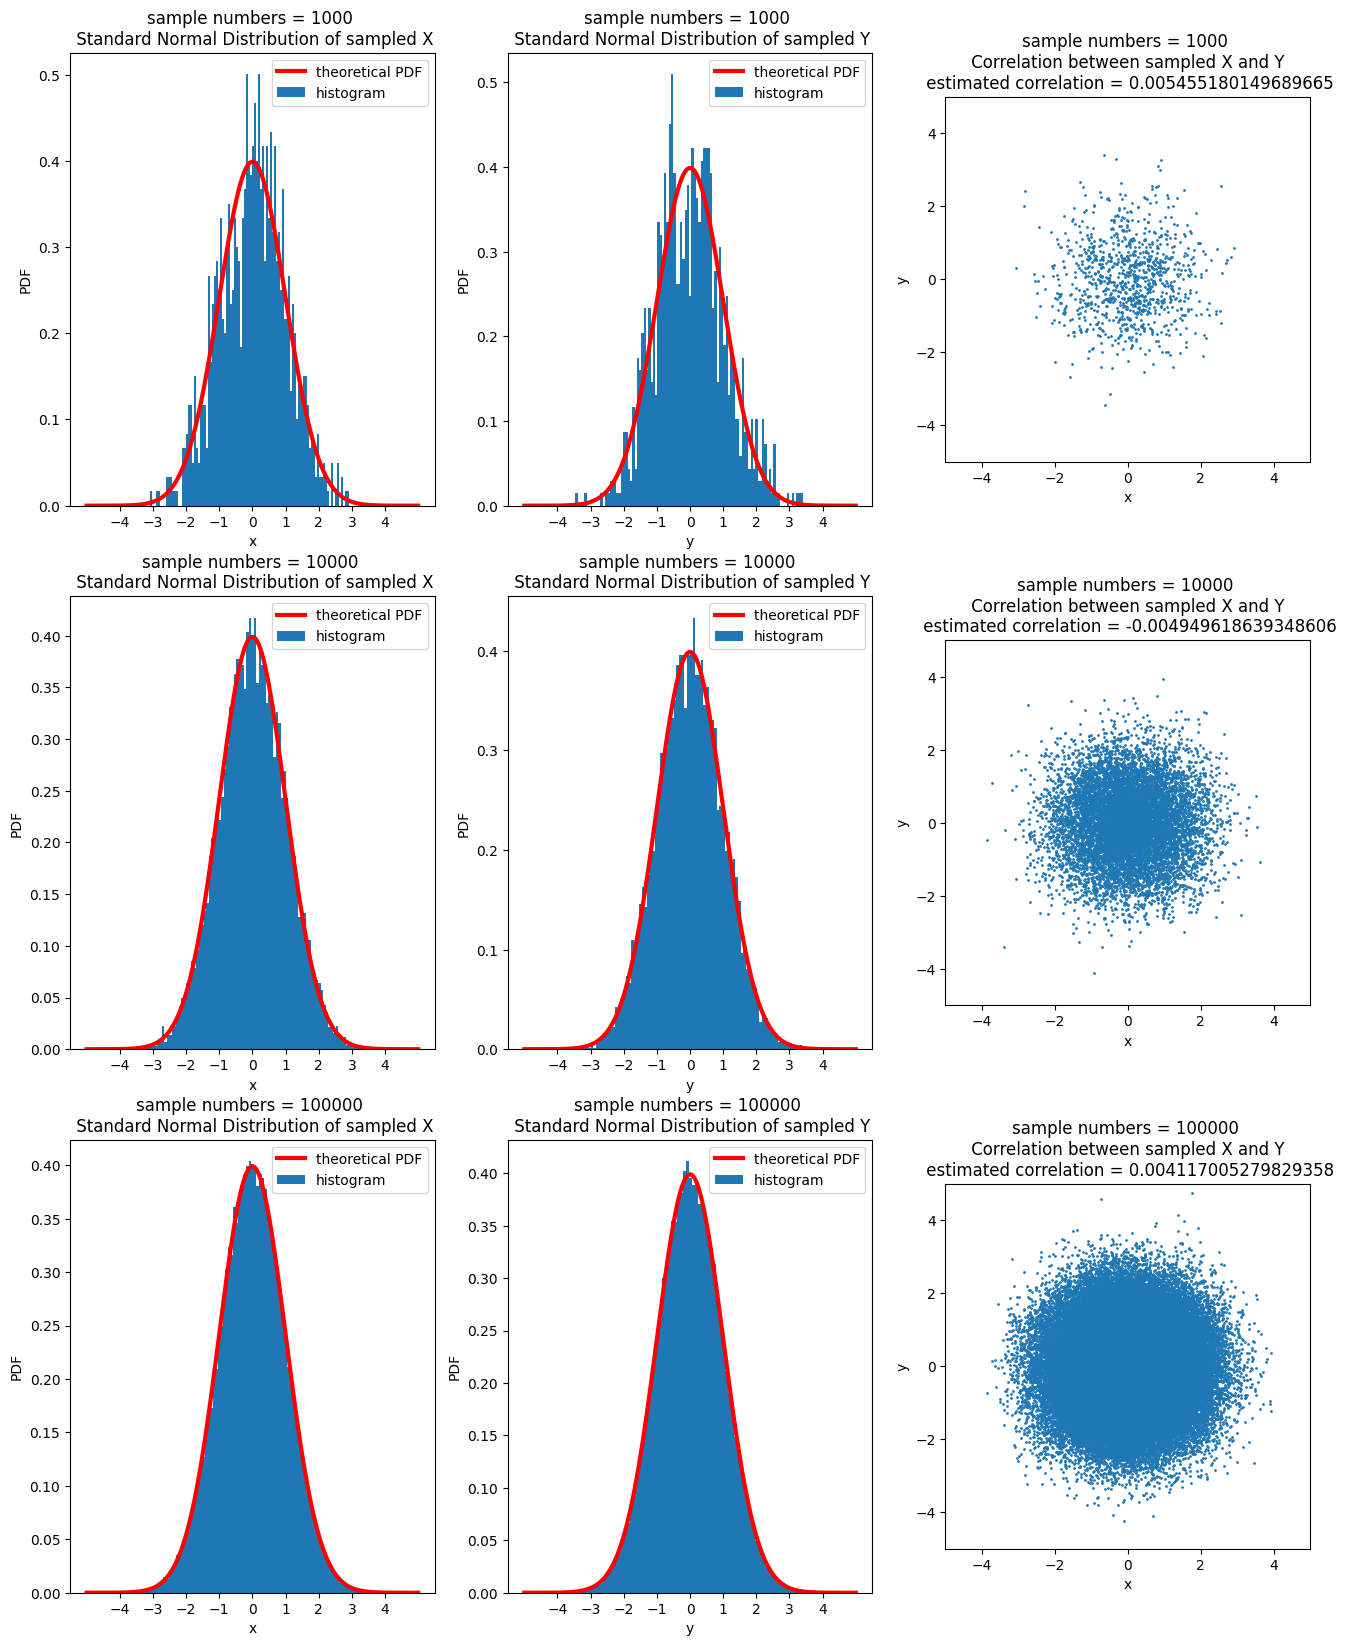
\includegraphics[width=0.8\textwidth]{./figure/p4/box_muller.png}
\end{figure}

(d) 1. Metropolis-Hastings Algorithm: \\
Advantages: It is highly general-purpose, could applicable to a wide variety of distributions, and it does not require the normalization constant of the target distribution. \\
Disadvantages: Samples are often requires select a suitable distribution, and requires steps to burn up.

2. Hamiltonian Monte Carlo Algorithm: \\
Advantages: Due to the conservation of energy, the acceptance rate should be $1$. But there exists numerical error, however quite close to $1$, which means it has quite high acceptance rate. The samples are efficient, especially in high-dimensional problems. \\
Disadvantages: Requires computation of gradients, increasing implementation complexity. Sensitive to parameters: step size $\delta$ and number of steps for LeapFrog $L$.

3. Box-Muller Method: \\
Advantages: Direct and simple method to generate independent standard normal samples, which is easy to implement. \\
Disadvantages: It would sample the normal distribution only.

\end{homeworkProblem}

\newpage
\begin{homeworkProblem}

\textbf{Beta Normal Distribution:} generate samples from the beta distribution $\Beta(5,5)$

(a) Implement a Metropolis-Hastings algorithm.

(b) Implement a Hamiltonian Monte Carlo algorithm.

(c) Implement with the Acceptance-Rejection Method.

(d) Compare the above three algorithms with corresponding pros and cons.

\solution

Let $X\sim \Beta(5,5)$. We can calculate the beta integral:
$$\beta(5,5)=\dfrac{\Gamma(5)\cdot\Gamma(5)}{\Gamma(10)}=\dfrac{4!\cdot 4!}{9!}=\dfrac{1}{630}$$
Then we can calculate the PDF of $X$:
$$f(x)=f_X(x)=\dfrac{1}{\beta(5,5)}x^{5-1}(1-x)^{5-1}=630x^4(1-x)^4 ,0<x<1$$

(a) Since the support of Beta distributio is $[0,1]$, so we can choose the proposal distribution to be $\Unif(1)$, which means that the one-step transition probability density from state $x$ to $y$ is $f_{x,y}=1$, thus we can get that the acceptance rate:
$$a_{x,y}=\min\left(\dfrac{\pi_jf_{j,i}}{\pi_if_{i,j}},1\right)=\min\left(\dfrac{j^4(1-j)^4}{i^4(1-i)^4},1\right)$$
Then we can do the Discrete time continuous state Metropolis-Hastings algorithm to sample the distribution $\Beta(5,5)$ in 1000000 samples, and the burn in is set to be 10000 samples. The result is as follows:
\begin{figure}[h]
    \centering
    \includegraphics[width=0.5\textwidth]{./figure/p5/MH.png}
\end{figure}

(b) Since $\pi_x$ is a the stationary distribution $\Beta(5,5)$, and we can ignore the constant form, so the potential energy is
$$U(x)=-\log(\pi_x) = -\log(630) -4\log(x(1-x)) \stackrel{\text{ignore const}}{\Rightarrow} U(x)=-4\log(x(1-x))$$
And let the mass be 1, then the Kinetic energy is
$$V(\omega)=\dfrac{1}{2}\omega^2, \quad\text{where } \omega\sim\N(0,1)$$
Thus the Hamiltonian energy is
$$H(x,\omega)=U(x)+V(\omega)=-4\log(x(1-x))+\dfrac{1}{2}\omega^2$$
Initially, set $x_0=0.5, \omega_0\sim\N(0,1)$, apply the Leapfrog method to sample:
\begin{align*}
\omega_{t+\frac{\delta}{2}} &= \omega_t - \frac{\delta}{2}\cdot \dfrac{\dU(x_t)}{\dx_t} = \omega_t - \frac{\delta}{2}\cdot \left(-\dfrac{4}{x_t}+\dfrac{4}{1-x_t}\right) \\
x_{t+\delta} &= x_t + \delta \cdot \dfrac{\dV(\omega_{t+\frac{\delta}{2}})}{\domega_{t+\frac{\delta}{2}}} = x_t + \delta\cdot \omega_{t+\frac{\delta}{2}} \\
\omega_{t+\delta} &= \omega_{t+\frac{\delta}{2}} - \frac{\delta}{2}\cdot \dfrac{\dU(x_{t+\delta})}{\dx_{t+\delta}} = \omega_{t+\frac{\delta}{2}} - \frac{\delta}{2}\cdot \left(-\dfrac{4}{x_{t+\delta}}+\dfrac{4}{1-x_{t+\delta}}\right)
\end{align*}
Due to the range limitation of $x\in(0,1)$, we can add a reflection bound at $x=0$ and $x=1$, i.e. when applying Leapfrog, if $x<0$, then set $x\gets -x, \omega\gets -\omega$, if $x>1$, then set $x\gets 2-x, \omega\gets -\omega$. After Leapfrog $L$ steps, we can get the state $(x_L, \omega_L)$. And set $(x_L, -\omega_L)$ to be the proposal distribution. And the accept rate for the Hamiltonian Monte Carlo algorithm is
$$a_{(x_0,\omega_0),(x_L,-\omega_L)}=\min\left(\dfrac{\exp\left(-H(x_L,-\omega_L)\right)}{\exp\left(-H(x_0,\omega_0)\right)}, 1\right)=\min\left(\dfrac{\exp\left(-U(x_L)-V(-\omega_L)\right)}{\exp\left(-U(x_0)-V(\omega_0)\right)}, 1\right)$$
We step the stepsize to be $\delta=0.05, L=15$, additionally, since the support is $(0,1)$, so for numerical accuracy, we clip x into the range $[10^{-10},1-10^{-10}]$. One trajectory and sample results are as follows:
\begin{figure}[h]
    \centering
    \includegraphics[width=0.5\textwidth]{./figure/p5/trajectory.png}
    \includegraphics[width=0.5\textwidth]{./figure/p5/Hamiltonian.png}
\end{figure}

(c) As for the acceptance-rejection algorithm, since the support of Beta distribution is $(0,1)$, so we can take $Y\sim \Unif(0,1)$. And its PDF is $g(y)=f_Y(y)=1$. \\
Let $c$ donate a constant:
$$c = \sup_y\dfrac{f(y)}{g(y)} = \sup_y\dfrac{20y(1-y)^3}{1}=630x^4(1-x)^4\big|_{y=\frac{1}{2}}=\dfrac{315}{128}$$
Then we can apply the Acceptance-Rejection algorithm to generate the samples on $X\sim \Beta(5,5)$:
\begin{figure}[h]
    \centering
    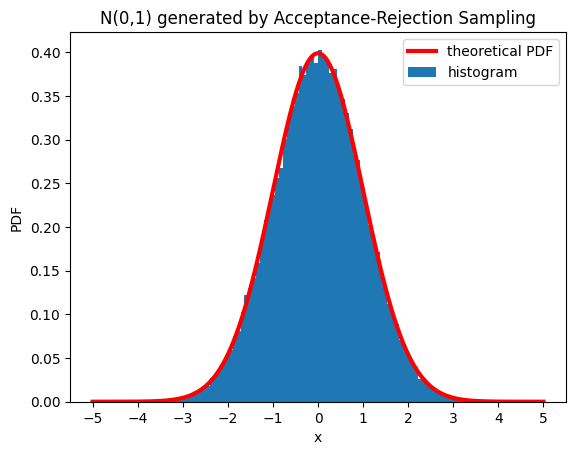
\includegraphics[width=0.5\textwidth]{./figure/p5/accept_reject.png}
\end{figure}

(d) 1. Metropolis-Hastings Algorithm: \\
Advantages: It is highly general-purpose, could applicable to a wide variety of distributions, and it does not require the normalization constant of the target distribution. \\
Disadvantages: Samples are often requires select a suitable distribution, and requires steps to burn up.

2. Hamiltonian Monte Carlo Algorithm: \\
Advantages: Due to the conservation of energy, the acceptance rate should be $1$. But there exists numerical error, however quite close to $1$, which means it has quite high acceptance rate. The samples are efficient, especially in high-dimensional problems. \\
Disadvantages: Requires computation of gradients, increasing implementation complexity. Sensitive to parameters: step size $\delta$ and number of steps for LeapFrog $L$.

3. Acceptance-Rejection Method: \\
Advantages: It produces independent samples, and is simple to implement. If the good envelope function is suitable, it is efficient. \\
Disadvantages: Efficiency depends heavily on the choice of proposal distribution, for example, ours implement has a quite low acceptance rate, which is only 0.0038838.

\end{homeworkProblem}

\newpage
\begin{homeworkProblem}

Given a random variable $X \sim \N(0,1)$, evaluate the tail probability $c=P(X>8)$ by Monte Carlo methods with \& without importance sampling. Discuss the pros and cons of importance sampling.

\textcolor{blue}{Solution} \\

1. Without importance sampling. \\
The total $10^9$ samples from $\N(0,1)$ have no single sample greater than 8. \\
So the tail probability estimatied is $c=P(X>8)=0$. \\

2. With importance sampling. \\
To calculate $c=P(Y>8)$, where $Y\sim \N(0,1)$. \\
So the PDF of $Y$ is that $f(y)=\dfrac{1}{\sqrt{2\pi}}e^{-\frac{1}{2}y^2}$. \\
It may be difficult to calculate the exact value of $c$ using simple sampling methods (because of the 3$\sigma$'s principle, the result must be very small). \\
So we can use the importance sampling. \\
Take $g\sim \N(8,1)$. \\
Let $Y_1,\cdots,Y_N\sim g$, so the PDF of $g$ is that $g(y_j)=\dfrac{1}{\sqrt{2\pi}}e^{-\frac{1}{2}(y_j-8)^2}$. \\
Let $h(Y_j)$ be the indicator that whether $Y_j>8$. \\

So with monty carlo method, we can get that \\
$$c=P(Y>8)=\E[\I(Y>8)]=\dfrac{1}{n}\sum_{j=1}^n\I(Y_j'>8)=\dfrac{1}{n}\sum_{j=1}^nh(Y_j')$$
where $Y_j'\sim \N(0,1)$.\\

With importance sampling, since
$$I=\E_f[h(Y)]=\int h(y)f(y)dy=\int\dfrac{h(y)f(y)}{g(y)}g(y)dy=E_g\left[\dfrac{h(Y)f(Y)}{g(Y)}\right]$$
So $I'=\dfrac{1}{n}\sum\limits_{i=1}^n\dfrac{h(Y_j)f(Y_j)}{g(Y_j)}$, where $Y_j\sim \N(8,1)$.\\
we can get that
\begin{align*}
c' &= \dfrac{1}{n}\sum_{j=1}^n\dfrac{h(Y_j)f(Y_j)}{g(Y_j)} \\
&= \dfrac{1}{n}\sum_{j=1}^n\I(Y_j>8)\cdot \dfrac{\frac{1}{\sqrt{2\pi}}e^{-\frac{1}{2}Y_j^2}}{\frac{1}{\sqrt{2\pi}}e^{-\frac{1}{2}(Y_j-8)^2}} \\
&= \dfrac{1}{n}\sum_{j=1}^n\I(Y_j>8)\cdot e^{-8Y_j+32}
\end{align*}

So we just need to sample $n$ times, $Y_j\sim \N(0,8)$, and calculate the average of $\I(Y_j>8)\cdot e^{-8Y_j+32}$.\\

The result using important sampling method is $6.252836307280847e-16$. \\
Which is very close to the correct answer $6.25*10^{-16}$. \\
So we can regard that the importance sampling method is effective and provide correct answers. \\

The following are the pages from jupyter notebook to show that the code can successful run out the images and calculation results we mentioned above. \\



3. The pros and cons of importance sampling. \\
Pros of Importance Sampling:
\begin{itemize}
    \item It is efficient because it allows sampling from a distribution that is easier to sample from, which simplifies the sampling process.
    \item It improves accuracy for rare events, provides more accurate estimates when dealing with low-probability tail.
\end{itemize}
Cons of Importance Sampling:
\begin{itemize}
    \item It depends on the choice of the proposal distribution. A poor choice can lead to high variance and inaccurate results.
    \item It requires more computations to calculate importance weights.
\end{itemize}

\end{homeworkProblem}

\newpage
\begin{homeworkProblem}

Generate uniform distributions over the following geometric objects: \\
(a) Ellipse $(a=2, b=1)$:
$$E_2(a, b)=\left\{(x, y) \in \mathbb{R}^2:\left(\frac{x}{a}\right)^2+\left(\frac{y}{b}\right)^2 \leq 1\right\}$$

(b) Sphere $(r=1)$:
$$S_2(r)=\left\{(x, y, z) \in \mathbb{R}^3: x^2+y^2+z^2=r^2\right\}$$

(c) Ball $(r=1)$:
$$B_3(r)=\left\{(x, y, z) \in \mathbb{R}^3: x^2+y^2+z^2 \leq r^2\right\}$$

(d) Torus $\left(r_0=2, r=1\right)$:
$$T_2\left(r_0, r\right)=\left\{(x, y, z) \in \mathbb{R}^3:\left(r_0-\sqrt{x^2+y^2}\right)^2+z^2=r^2\right\}$$

\textcolor{blue}{Solution} \\

(a) 1. Acceptance-Rejection method: \\
\begin{figure}[h]
    \centering
    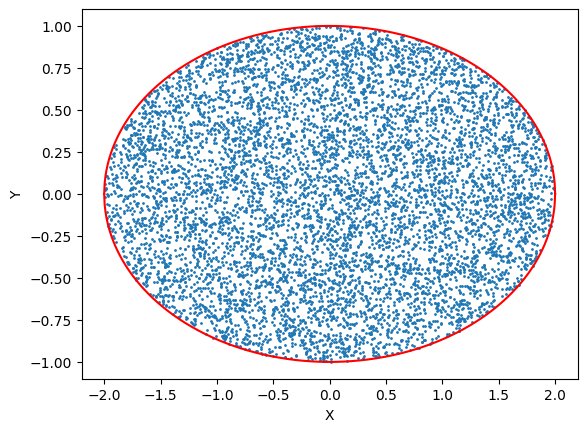
\includegraphics[width=0.8\textwidth]{./figure/p7/a_accept_reject.png}
    \caption{Ellipse sample by Acceptance-Rejection method}
\end{figure}

2. Change of variable: \\
Let $x=a\cdot r\cos\theta$, $y=b\cdot r\sin\theta$, where $\theta\in [0, 2\pi], r\in [0, 1]$. The Jacobian is $|J|=\left|\dfrac{\partial(x, y)}{\partial(r, \theta)}\right|=abr$.

Since the area of the ellipse is $\pi ab$, so the PDF of the ellipse is $f_{X, Y}(x, y)=\dfrac{1}{\pi ab}$. Thus we have
$$f_{R, \Theta}(r, \theta)=f_{X, Y}(x, y)\cdot|J|=\dfrac{1}{\pi ab}\cdot abr=\dfrac{r}{\pi}=f_R(r)f_{\Theta}(\theta)$$
So $R$ and $\Theta$ are independent variables, we can sample them respectively.
\begin{align*}
f_R(r) &= \int_{0}^{2\pi}f_{R, \Theta}(r, \theta)d\theta = 2r \\
F_R(r) &= \int_{0}^{r}f_R(r)dr = r^2 \\
F^{-1}_R(u) &= \sqrt{u} \\
f_{\Theta}(\theta) &= \int_{0}^{1}f_{R, \Theta}(r, \theta)dr = \dfrac{1}{2\pi} \\
F_{\Theta}(\theta) &= \int_{0}^{\theta}f_{\Theta}(\theta)d\theta = \dfrac{\theta}{2\pi} \\
F^{-1}_{\Theta}(u) &= 2\pi u
\end{align*}

$U_1, U_2\stackrel{i.i.d.}{\sim} \Unif(0, 1)$, then let
$$r\leftarrow \sqrt{U_1}, \theta\leftarrow 2\pi U_2$$
Then $(X, Y)$ can be uniformly sampled from the ellipse.
$x = a\cdot r\cos\theta = 2\sqrt{U_1}\cos(2\pi U_2)$, $y = b\cdot r\sin\theta = \sqrt{U_1}\sin(2\pi U_2)$
\begin{figure}[h]
    \centering
    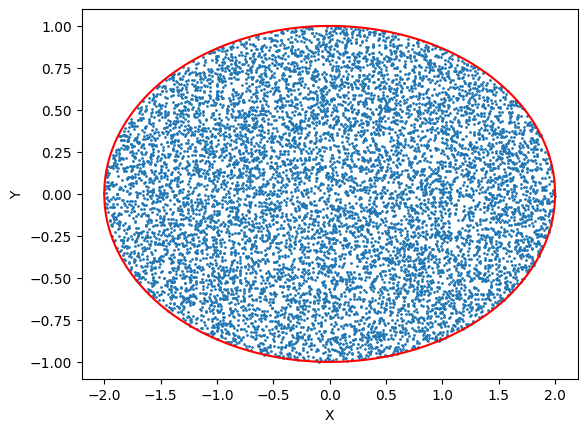
\includegraphics[width=0.8\textwidth]{./figure/p7/a_change_variable.png}
    \caption{Ellipse sample by Change of variable}
\end{figure}


(b) Let $x=r\sin\theta\cos\phi$, $y=r\sin\theta\sin\phi$, $z=r\cos\theta$, where $\theta\in [0, \pi], \phi\in [0, 2\pi]$. The Jacobian is $J=\dfrac{\partial(x, y, z)}{\partial(\theta, \phi)}=\begin{pmatrix}
r\cos\theta\cos\phi & -r\sin\theta\sin\phi \\
r\cos\theta\sin\phi & r\sin\theta\cos\phi \\
-r\sin\theta & 0
\end{pmatrix}$
The Gram matrix $G=J^{\top}J=\begin{pmatrix}
r^2 & 0 \\
0 & r^2\sin^2\theta
\end{pmatrix}$.
The area of the sphere is $4\pi r^2$, so the PDF of the sphere is $f_{X, Y, Z}(x, y, z)=\dfrac{1}{4\pi r^2}$.
So we have
$$f_{\Theta, \Phi}(\theta, \phi) = f_{X, Y, Z}(x, y, z)\cdot|\sqrt{\det(G)}|=\dfrac{1}{4\pi r^2}\cdot r^2\sin\theta = \dfrac{1}{4\pi}\sin\theta=f_{\Theta}(\theta)f_{\Phi}(\phi)$$
So $\Theta$ and $\Phi$ are independent variables, we can sample them respectively.
\begin{align*}
f_{\Theta}(\theta) &= \int_{0}^{2\pi}f_{\Theta, \Phi}(\theta, \phi)d\phi = \dfrac{1}{2}\sin\theta \\
F_{\Theta}(\theta) &= \int_{0}^{\theta}f_{\Theta}(\theta)d\theta = \dfrac{1-\cos\theta}{2} \\
F^{-1}_{\Theta}(u) &= \arccos(1-2u) \\
f_{\Phi}(\phi) &= \int_{0}^{\pi}f_{\Theta, \Phi}(\theta, \phi)d\theta = \dfrac{1}{2\pi} \\
F_{\Phi}(\phi) &= \int_{0}^{\phi}f_{\Phi}(\phi)d\phi = \dfrac{\phi}{2\pi} \\
F^{-1}_{\Phi}(u) &= 2\pi u
\end{align*}

Sample $U_1, U_2\stackrel{i.i.d.}{\sim} \Unif(0, 1)$, then let
$$\theta\leftarrow \arccos(1-2U_1), \phi\leftarrow 2\pi U_2$$
Since $\cos\theta = 1 - 2U_1$, and $\theta\in [0, \pi]$, so $\sin\theta = 2\sqrt{U_1(1-U_1)}$. Then we set that
$$x\gets r\sin\theta\cos\phi = 2\sqrt{U_1(1-U_1)}\cos(2\pi U_2), y\gets r\sin\theta\sin\phi = 2\sqrt{U_1(1-U_1)}\sin(2\pi U_2), z\gets r\cos\theta = 1-2U_1$$
Then $(X, Y, Z)$ can be uniformly sampled from the sphere.

\begin{figure}[ht]
    \centering
    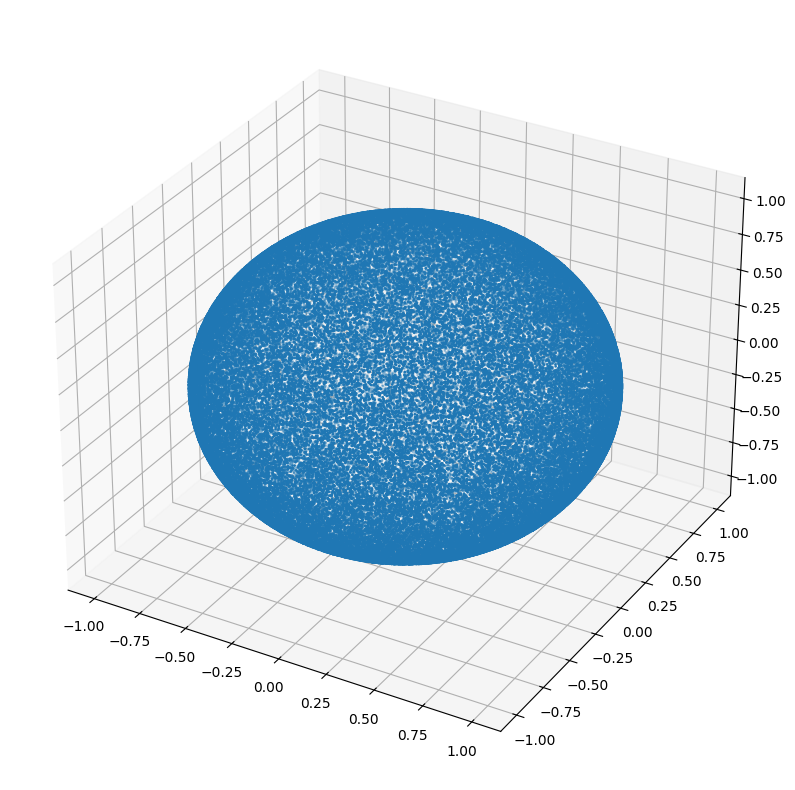
\includegraphics[width=0.48\textwidth]{./figure/p7/b_sample.png}
    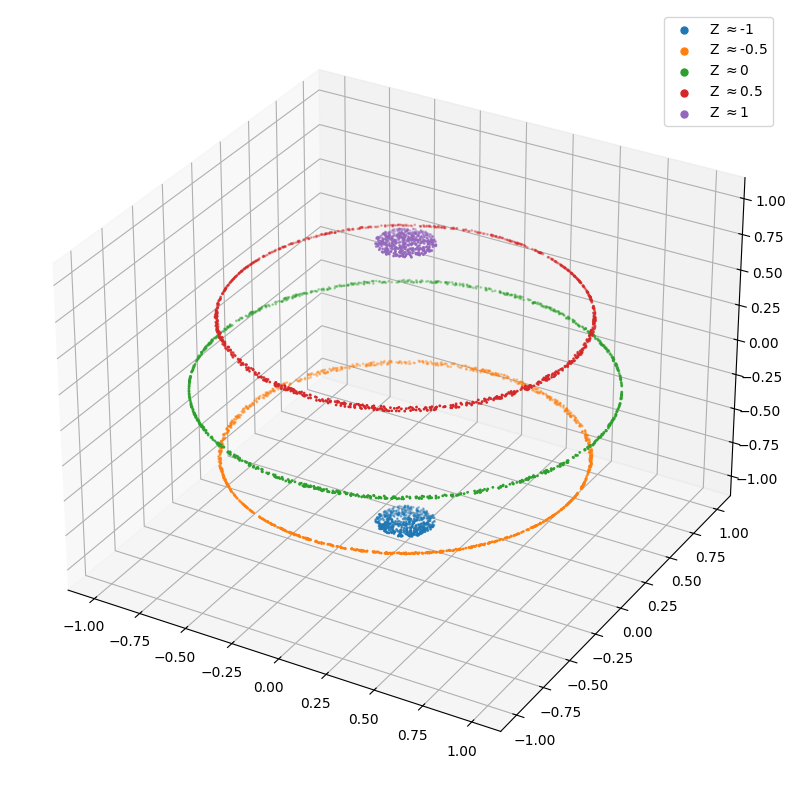
\includegraphics[width=0.48\textwidth]{./figure/p7/b_contour.png}
    \caption{Left: Sphere's sample points. Right: Some contours of the Sphere to show the inner details.}
\end{figure}


(c) Let $x=r\sin\theta\cos\phi$, $y=r\sin\theta\sin\phi$, $z=r\cos\theta$, where $\theta\in [0, \pi], \phi\in [0, 2\pi], r\in [0, 1]$. The Jacobian is $J=\dfrac{\partial(x, y, z)}{\partial(r, \theta, \phi)}=r^2\sin\theta$.

Since the volume of the ball is $\dfrac{4}{3}\pi r^3=\dfrac{4}{3}\pi$, so the PDF of the ball is $f_{X, Y, Z}(x, y, z)=\dfrac{3}{4\pi}$. Thus we have
$$f_{R, \Theta, \Phi}(r, \theta, \phi)=f_{X, Y, Z}(x, y, z)\cdot|J|=\dfrac{3}{4\pi}\cdot r^2\sin\theta=f_R(r)f_{\Theta}(\theta)f_{\Phi}(\phi)$$
So $R$, $\Theta$ and $\Phi$ are independent variables, we can sample them respectively.

\begin{align*}
f_R(r) &= \int_{0}^{2\pi}\int_{0}^{\pi}f_{R, \Theta, \Phi}(r, \theta, \phi)d\theta d\phi = 3r^2 \\
F_R(r) &= \int_{0}^{r}f_R(r)dr = r^3 \\
f_{\Theta}(\theta) &= \int_{0}^{2\pi}\int_{0}^{1}f_{R, \Theta, \Phi}(r, \theta, \phi)dr d\phi = \dfrac{1}{2}\sin\theta \\
F_{\Theta}(\theta) &= \int_{0}^{\theta}f_{\Theta}(\theta)d\theta = \dfrac{1}{2}(1-\cos\theta) \\
f_{\Phi}(\phi) &= \int_{0}^{2\pi}\int_{0}^{1}f_{R, \Theta, \Phi}(r, \theta, \phi)dr d\theta = \dfrac{1}{2\pi} \\
F_{\Phi}(\phi) &= \int_{0}^{\phi}f_{\Phi}(\phi)d\phi = \dfrac{\phi}{2\pi}
\end{align*}

$U_1, U_2, U_3\stackrel{i.i.d.}{\sim} \Unif(0, 1)$, then let
$$r\leftarrow \sqrt[3]{U_1}, \theta\leftarrow \arccos(1-2U_2), \phi\leftarrow 2\pi U_3$$
We can ree-write $\cos\theta=1-2U_2$, and $\sin\theta=2\sqrt{U_2(1-U_2)}$ to save computational complexity.
Then $(X, Y, Z)$ can be uniformly sampled from the ball.

\begin{figure}[ht]
    \centering
    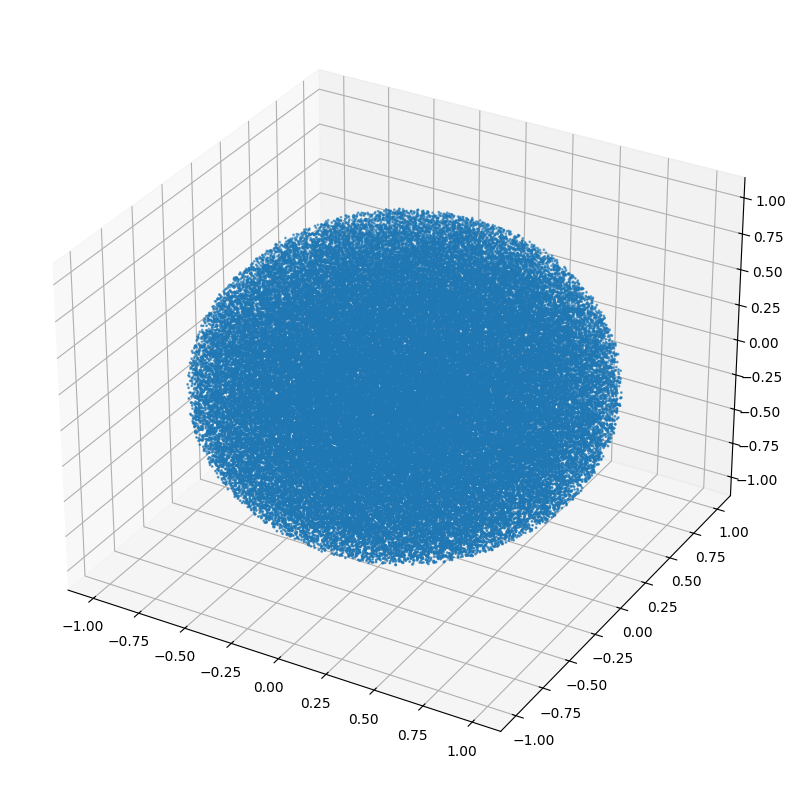
\includegraphics[width=0.48\textwidth]{./figure/p7/c_sample.png}
    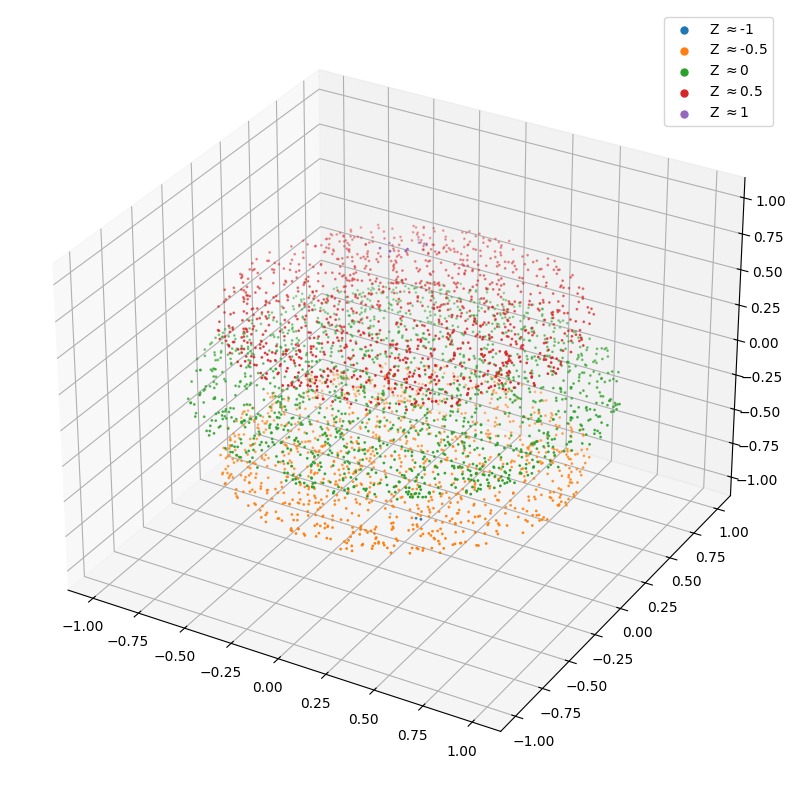
\includegraphics[width=0.48\textwidth]{./figure/p7/c_contour.png}
    \caption{Left: Ball's sample points. Right: Some contours of the Ball to show the inner details.}
\end{figure}


(d) Let $x=(r_0+r\cos\theta)\cos\phi, y=(r_0+r\cos\theta)\sin\phi, z=r\sin\theta$, where $\theta\in [0, 2\pi], \phi\in [0, 2\pi], r\in [0, 1]$. The Jacobian is $J=\dfrac{\partial(x, y, z)}{\partial(r, \theta, \phi)}=\begin{pmatrix}
-r\sin\theta\cos\phi & -(r_0+r\cos\theta)\sin\phi \\
-r\sin\theta\sin\phi & (r_0+r\cos\theta)\cos\phi \\
r\cos\theta & 0
\end{pmatrix}$.
So the Gram matrix $G=J^{\top}J=\begin{pmatrix}
r^2 & 0 \\
0 & (r_0+r\cos\theta)^2
\end{pmatrix}$.
Since $r=1$, so $r\cos\theta>0$

$$\dS = \sqrt{\det(G)}\dtheta\dphi = r(r_0+r\cos\theta)\dr\dtheta\dphi$$
\begin{align*}
S &= \oint \dS \\
&= \int_{0}^{2\pi}\int_{0}^{2\pi}r(r_0+r\cos\theta)d\theta d\phi \\
&= 4\pi^2r\cdot r_0 \\
&= 8\pi^2
\end{align*}
$f_{X,Y,Z}(x,y,z)=\dfrac{1}{4\pi^2r\cdot r_0}=\dfrac{1}{8\pi^2}$, so
$$f_{\Theta, \Phi}(\theta,\phi)=\dfrac{1}{4\pi^2r_0}\cdot r(r_0+r\cos\theta)=\dfrac{r_0+r\cos\theta}{4\pi^2r_0} = \dfrac{2+\cos\theta}{8\pi^2}=f_{\Theta}(\theta)f_{\Phi}(\phi)$$
So $\Theta$ and $\Phi$ are independent variables, we can sample them respectively.

\begin{align*}
f_{\Theta}(\theta) &= \int_{0}^{2\pi}f_{\Theta, \Phi}(\theta,\phi)d\phi = \dfrac{r_0+r\cos\theta}{2\pi r_0} = \dfrac{2+\cos\theta}{4\pi} \\
F_{\Theta}(\theta) &= \int_{0}^{\theta}f_{\Theta}(\theta)d\theta = \dfrac{1}{2\pi}\theta + \dfrac{r}{2\pi r_0}\sin\theta = \dfrac{1}{2\pi}\theta + \dfrac{1}{4\pi}\sin\theta \\
f_{\Phi}(\phi) &= \int_{0}^{2\pi}f_{\Theta, \Phi}(\theta,\phi)d\theta = \dfrac{1}{2\pi} \\
F_{\Phi}(\phi) &= \int_{0}^{\phi}f_{\Phi}(\phi)d\phi = \dfrac{\phi}{2\pi}
\end{align*}

$U_1, U_2\stackrel{i.i.d.}{\sim} \Unif(0, 1)$, then let
$\theta$ be the solution that $\dfrac{1}{2\pi}\theta + \dfrac{1}{4\pi}\sin\theta=U_1$, $\phi\leftarrow 2\pi U_2$. $\theta$ has no closed form solution, but we can use the toolkits to solve the equation as the valid CDF must exist a solution.

Then $(X, Y, Z)$ can be uniformly sampled from the Torus whose $r_0=2,r=1$.

\begin{figure}[ht]
    \centering
    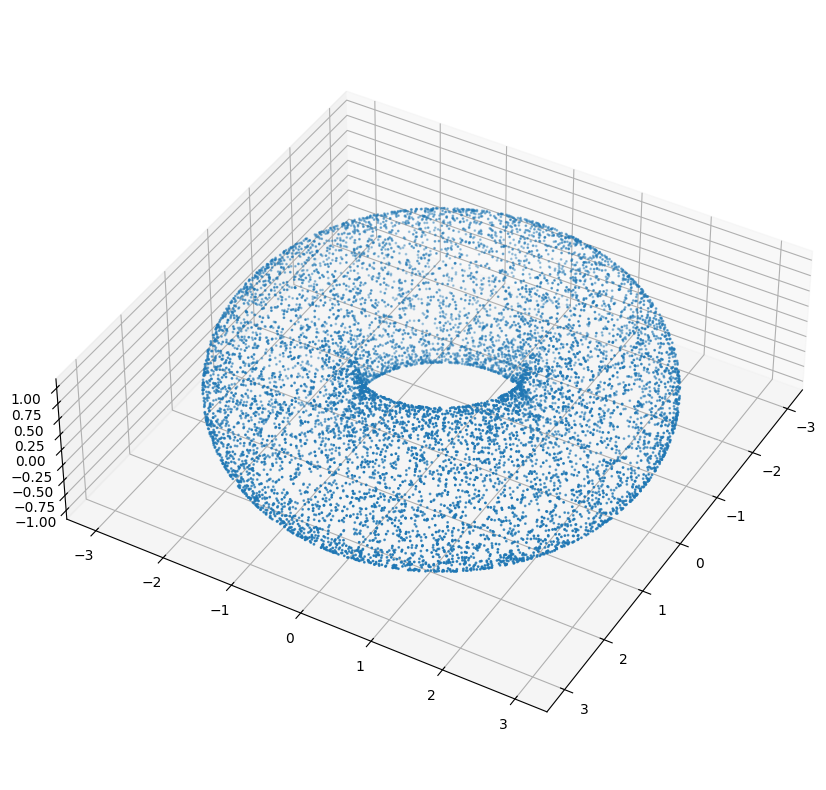
\includegraphics[width=0.48\textwidth]{./figure/p7/d_sample.png}
    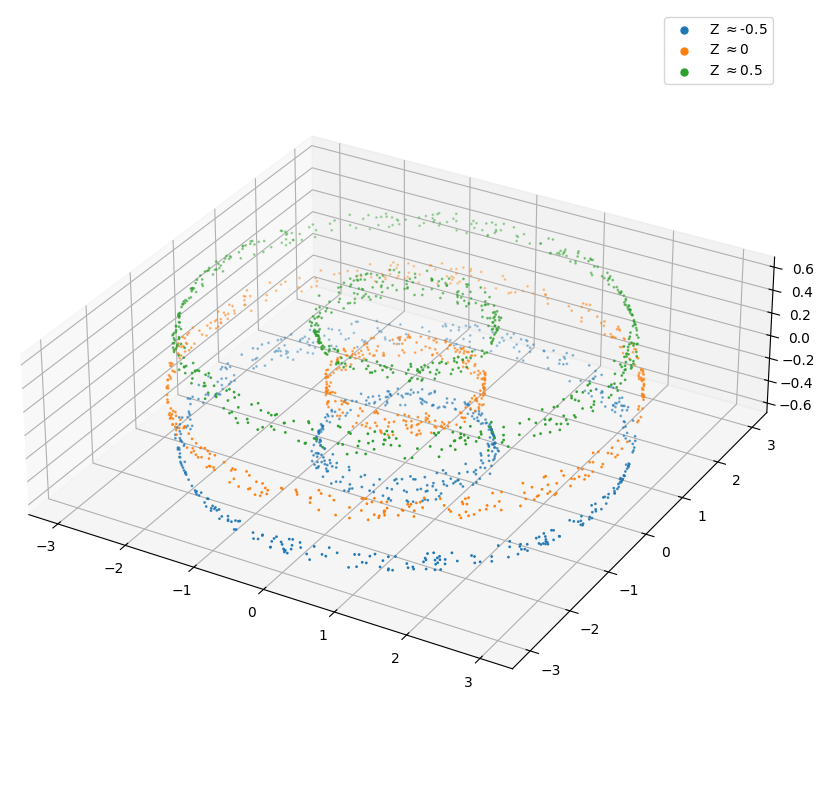
\includegraphics[width=0.48\textwidth]{./figure/p7/d_contour.png}
    \caption{Left: Torus's sample points. Right: Some contours of the Torus to show the inner details.}
\end{figure}

\end{homeworkProblem}

\newpage
\begin{homeworkProblem}

\textbf{Chicken-Egg with Unknown Parameters:} The parameter setting: $\lambda=10, a=b=1, x=7$.

(a) Implement a Gibbs sampler to find the posterior mean and the variance of $p$ after observing $x$ hatched eggs.

(b) Implement a Metropolis-Hastings algorithm to find the posterior mean and variance of $p$ after observing $x$ hatched eggs.

(c) Compare such two methods of MCMC.

\solution

Let $N\sim\Pois(\lambda)$ donates number of eggs. \\
The prior distribution of the hatch probability is $P\sim\Beta(a,b)$. \\
$X|P=p\sim\Pois(\lambda p)$ is the number of hatched eggs, $N-X|P=p\sim\Pois(\lambda(1-p))$ is the number of unhatched eggs.

(a) Directly sample the conditional probability above is complex, so we consider the conditional joint distribution of $X,N|P$: \\
Since $X|N=n,P=p\sim\Bin(n,p)$, and we have the prior $P\sim\Beta(a,b)$, from the Beta-Binomial conjugate, we can get that
$$P|N=n,X=x\sim\Beta(a+x,b+n-x)$$
And from the definition of $N$ and $X$, we have
$$f_{N|P,X}(n|P=p,X=x) \sim x + \Pois(\lambda(1-p))$$
The conditional distributions are all easy to sample, so we can use the Gibbs sampling to sample the joint distribution of $P,N|X$, then the marginal distribution of $P|X=x$ and $N|X=x$ can be calculated. Set the initial state to be $p_0=0.5, n_0=7$.  The sampling results are as follows:
\begin{figure}[h]
    \centering
    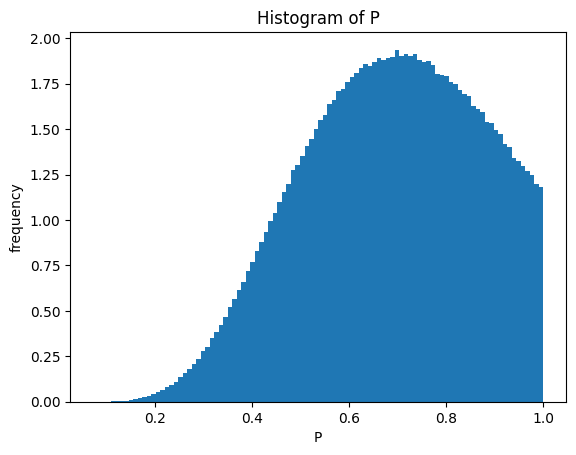
\includegraphics[width=0.49\textwidth]{./figure/p8/Gibbs_P.png}
    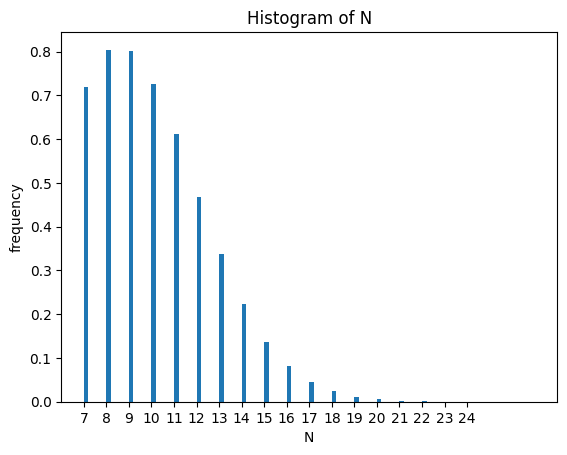
\includegraphics[width=0.49\textwidth]{./figure/p8/Gibbs_N.png}
\end{figure}

The estimated P given $X = 7$ has mean: $0.68449$, variance: $0.03196$.

(b) Directly calculate the posterior distribution of $P$ with Metropolis-Hastings algorithm:
\begin{align*}
f_{P|X}(p|X=x) &\propto P(X=x|P=p)f_P(p) \\
&= e^{-(\lambda p)}\dfrac{(\lambda p)^x}{x!} \cdot \dfrac{1}{\beta(a,b)}p^{a-1}(1-p)^{b-1} \\
&\propto e^{-\lambda p}(\lambda p)^x\cdot p^{a-1}(1-p)^{b-1}
\end{align*}
Since the support of $P$ is $[0,1]$, thus we can $\Unif(0,1)$ to be the proposal distribution, i.e. the one-step transition probability density from state $x$ to $y$ is $f_{i,j}=f_{X_{n+1}|X_n}(j|i)=1,j>0$, so we can get that the acceptance rate:
$$a_{i,j}=\min\left(\dfrac{\pi_jf_{j,i}}{\pi_if_{i,j}},1\right)=\min\left(\dfrac{e^{-\lambda j}(\lambda j)^x\cdot j^{a-1}(1-j)^{b-1}}{e^{-\lambda i}(\lambda i)^x\cdot i^{a-1}(1-i)^{b-1}},1\right)$$
The sampling results are as follows:
\begin{figure}[h]
    \centering
    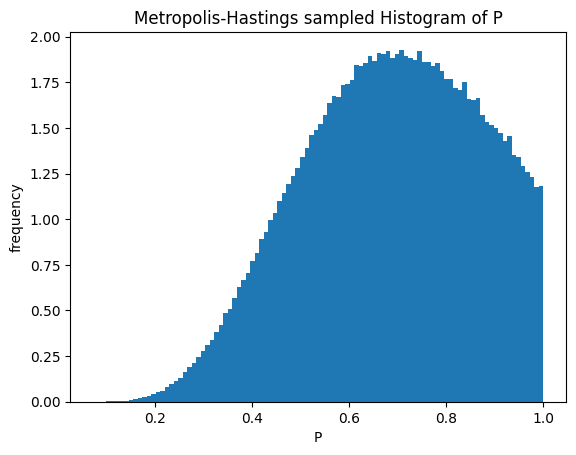
\includegraphics[width=0.6\textwidth]{./figure/p8/MH_P.png}
\end{figure}
The estimated P given $X = 7$ has mean: $0.68468$, variance: $0.03198$.

(c) We can see that both Gibbs sampling and Metropolis-Hastings algorithm with same sample number as burn in number have a similar estimation.

Metropolis-Hastings: \\
Advantages: It can sample many different distributions with suitable proposal distribution, without requiring the conditional distribution is easy to sample. \\
Disadvantages: It is actually a accept-reject method, if the simulation steps are not enough, it may reject many times and stay at the same state, also, it may need more calculations.


Gibbs sampling:
Advantages: It need less calculations, do not need to reject samples, thus it is efficient. \\
Disadvantages: It need to sample the conditional distribution, which required to be easy to sample. If the conditional distributions are complex, it still require Metropolis-Hastings algorithm or other sampling methods to generate a single sample, which is not efficient.

\end{homeworkProblem}

\newpage
\begin{homeworkProblem}

\textbf{Three-dimensional Joint Distribution:} Implement a Gibbs sampler to generate samples from the three-dimensional joint distribution shown in the lecture.

\solution

Random variables $X,P,N$ have joint density
$$\pi(x,p,n)\propto \binom{n}{x}p^x(1-p)^{n-1}\dfrac{4^n}{n!}$$
for $x=0,1,2,\ldots,n$, $0<p<1$, and $n=0,1,2,\ldots$. The $p$ variable is continuous, $x$ and $n$ are discrete. We can get the conditional PDF and PMF for the corresponding variables as follows:
\begin{align*}
P_{X|N,P}(X=x|N=n,P=p) &\propto \binom{n}{x}p^x(1-p)^{n-x}\sim \Bin(n,p) \\
f_{P|X,N}(p|X=x,N=n) &\propto p^x(1-p)^{n-x} \sim \Beta(x+1,n-x+1) \\
P_{N|X,P}(N=n|X=x,P=p) &\propto \binom{n}{x}p^x(1-p)^{n-x} = x + Z
\end{align*}
We can get that the last PMF is a shifted Poisson, where $Z\sim\Pois(4(1-p))$. \\
Initially, we set $(x_0,p_0,n_0)\gets(1,0.5,2)$, and we can use Gibbs sampling to generate the samples. \\
The simulated results are as follows:

\begin{figure}[h]
    \centering
    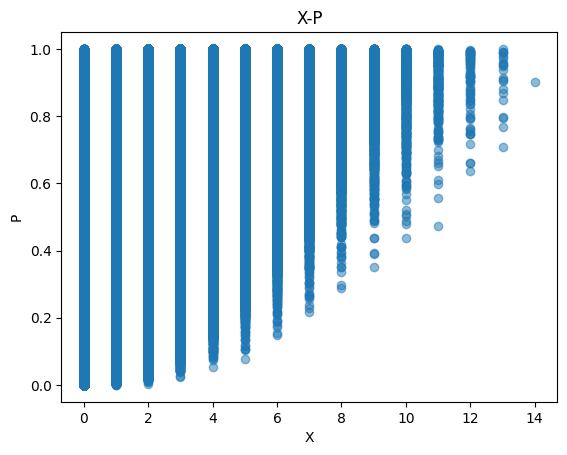
\includegraphics[width=0.4\textwidth]{./figure/p9/X_P.png}
    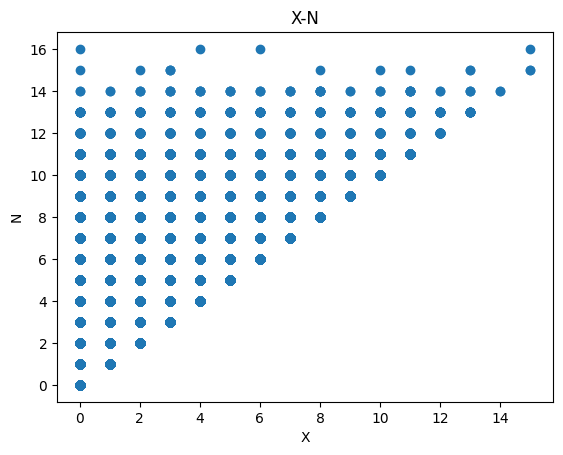
\includegraphics[width=0.4\textwidth]{./figure/p9/X_N.png}
\end{figure}
\begin{figure}[h]
    \centering
    \includegraphics[width=0.49\textwidth]{./figure/p9/P_N.png}
    \includegraphics[width=0.4\textwidth]{./figure/p9/X_P_N.png}
\end{figure}

\vspace{1cm}
The estimated marginal distribution are as follows:
\begin{figure}[h]
    \centering
    \includegraphics[width=0.4\textwidth]{./figure/p9/X.png}
\end{figure}
\begin{figure}[h]
    \centering
    \includegraphics[width=0.4\textwidth]{./figure/p9/P.png}
\end{figure}
\begin{figure}[h]
    \centering
    \includegraphics[width=0.4\textwidth]{./figure/p9/N.png}
\end{figure}

\end{homeworkProblem}

\newpage

\end{document}